\chapter{Análisis Experimental} \label{capitulo:analisis-experimental}
\markright{Análisis Experimental}

En este capítulo se presentan las decisiones tomadas en torno a las configuraciones de los clasificadores y el análisis de los resultados obtenidos durante los experimentos. 

\section{Decisiones de configuración} \label{capitulo:configuracion}

\paragraph{} Durante el análisis experimental fueron realizadas comparaciones entre las clasificaciones obtenidas por redes neuronales y SVM.
En particular, fue de interés estudiar el comportamiento de las redes neuronales y SVM en términos del tamaño del problema.

\paragraph{} Tomando el trabajo de \citet{savant-original} como inspiración, se optó por trabajar con clasificadores entrenados con una determinada dimensión del problema (en particular $512$ tareas sobre $16$ máquinas o $512\times 16$) a la hora de clasificar y evaluar instancias del problema con menor, igual y mayor cantidad de tareas.
Para hacer esto posible, se generaron instancias del problema de dimensión $512\times 16$, utilizadas para el entrenamiento de los clasificadores.
Así también, como se presentó en la Sección \ref{chapter-implementacion:data}, para cada dimensión del problema desde $17\times 16$ hasta $1024\times 16$, se generaron conjuntos de $10$ instancias del problema, las cuales fueron utilizadas para calcular y comparar la precisión en la clasificación para redes neuronales y SVM.

\newpage % orphaned line.

\paragraph{} Las redes neuronales fueron entrenadas con diferentes cantidades de capas ocultas, habiéndose generado con $2$, $3$ y $4$ capas ocultas, siendo 4 el máximo número de capas ocultas empleado debido a limitaciones de recursos y tiempos de entrenamiento altos.

\paragraph{} Como fue mencionado en el Capítulo \ref{chapter-implementation}, para obtener una primera selección de parámetros de configuración para el entrenamiento de las redes neuronales se utilizó el método \textit{GridSearch} de la clase \textit{model\_selection.GridSearchCV} de \textit{scikit-learn}.
Este método realiza una búsqueda, mediante validación cruzada, de los mejores parámetros para el entrenamiento de un clasificador.
Para eso es necesario definir conjuntos de posibles valores a ser utilizados en los parámetros de los clasificadores.
A continuación se presentan los valores considerados para cada uno de esos parámetros.
Para el parámetro  \textit{solver}, se consideraron el método de optimización de los pesos \textit{Broyden–Fletcher–Goldfarb–Shanno} para memoria limitada (\textit{lbfgs}), Gradiente Descendente (\textit{sgd}) y el método Adam (\textit{adam}).
Para el coeficiente de aprendizaje, llamado \textit{alpha}, se consideraron los valores \textit{0.01} y \textit{0.0001}.
Finalmente, para el parámetro \textit{activation}, que indica la función de activación utilizada, se consideraron las funciones \textit{relu}, \textit{tanh} e \textit{identity}.
Los resultados del método \textit{GridSearch} para los parámetros mencionados se muestran en la Tabla \ref{table:parametros}.
Con respecto al parámetro \textit{activation} se observó que el valor seleccionado por el método \textit{GridSearch} fue \textit{relu}; esto fue de particular interés debido a que dicha función de activación cambia de forma abrupta en su pendiente. Las primeras pruebas realizadas utilizando la red neuronal con activación \textit{relu}, brindaron resultados de \textit{makespan} mayores a los resultados de \textit{makespan} generados por SVM. 
Al variar la función de activación de la red neuronal, se obtuvieron resultados de \textit{makespan} menores a los valores de \textit{makespan} obtenidos con SVM.
Esto llevó a variar las funciones de activación para estudiar el comportamiento de las redes neuronales con funciones de activación con pendientes que no tuvieran cambios abruptos.
El resto de los parámetros se mantuvieron de acuerdo a los resultados del método \textit{GridSearch}.

\begin{table}[h!]
\centering
\begin{tabular}{ |p{0.25\linewidth}|p{0.25\linewidth}| } 
\hline
\textbf{Parámetro} & \textbf{Valor}\\
\hline
solver & lbfgs\\ 
\hline
alpha & 0.01\\ 
\hline
activation & relu\\ 
\hline
\end{tabular}
\caption{ Valores para los parámetros de las redes neuronales, obtenidos mediante el método \textit{GridSearch} de la biblioteca \textit{scikit-learn}}
\label{table:parametros}
\end{table}

\paragraph{} Se evaluaron las redes neuronales resultantes de las combinaciones de las funciones de activación \textit{relu}, \textit{tanh} e \textit{identity} y las cantidades de capas ocultas, profundizando en las pruebas para aquellas combinaciones que mostraban resultados más prometedores.

\section{Análisis combinado para redes neuronales de 2, 3 y 4 capas ocultas}

\paragraph{}En primer lugar fueron comparados los resultados de \textit{makespan} para soluciones obtenidas a partir de las redes neuronales, utilizando como funciones de activación a \textit{tanh}, \textit{identity} y \textit{relu}, con 2, 3 y 4 capas ocultas.
Asimismo, en esta comparación, también fueron analizados los resultados obtenidos con SVM. 

\paragraph{} Cada clasificador fue entrenado con 100 instancias del problema de dimensión $512\times16$, lo que se traduce en 51200 instancias de entrenamiento para los clasificadores. Para cada dimensión del rango estudiado, se utilizaron 10 instancias del problema para validar el rendimiento de las redes neuronales y SVM. Los resultados presentados en esta sección son promedios de los resultados individuales de estas 10 instancias.

\paragraph{} Fueron identificados aquellos clasificadores que obtuvieron mejores resultados en \textit{makespan}.
Las Figuras \ref{fig:relu234}, \ref{fig:identity234} y \ref{fig:tanh234} muestran las diferencias porcentuales de \textit{makespan} con respecto al \textit{makespan} obtenido por el algoritmo Min-Min, para la clasificación de instancias del problema en un rango de dimensiones que va desde $17\times16$ a $1024\times16$.

\paragraph{} De manera similar, los resultados también fueron agrupados de acuerdo a su dimensión.
Esta agrupación fue realizada de a 200 tareas con la excepción de que el primero y el último de los conjuntos van desde la dimensión $17\times16$ a $200\times16$ y $1000\times16$ a $1024\times16$, respectivamente.

\paragraph{}La Figura \ref{fig:relu234} muestra los resultados para las redes neuronales utilizando la función de activación \textit{relu}.
En dicha figura se observa que el \textit{makespan} obtenido por los resultados de la SVM se aproxima más al \textit{makespan} dado por los resultados del algoritmo Min-Min que para los resultados obtenidos con las redes neuronales, cualquiera sea la cantidad de capas ocultas utilizada. 

\paragraph{} Cabe destacar que a medida que aumenta la cantidad de capas ocultas de la red neuronal, los resultados se alejan de los valores esperados llegando, para clasificaciones sobre dimensiones pequeñas, a estar a más del $100\%$ por sobre los valores esperados.
Los mejores resultados de las redes neuronales se observan para aquellas redes neuronales con solo dos capas ocultas.
% TODO ¿agregar algo sobre que probablemente la función aprendida no requiere de la complejidad que permite una mayor cantidad de capas ocultas? 


\begin{figure}[H]
  \centering
  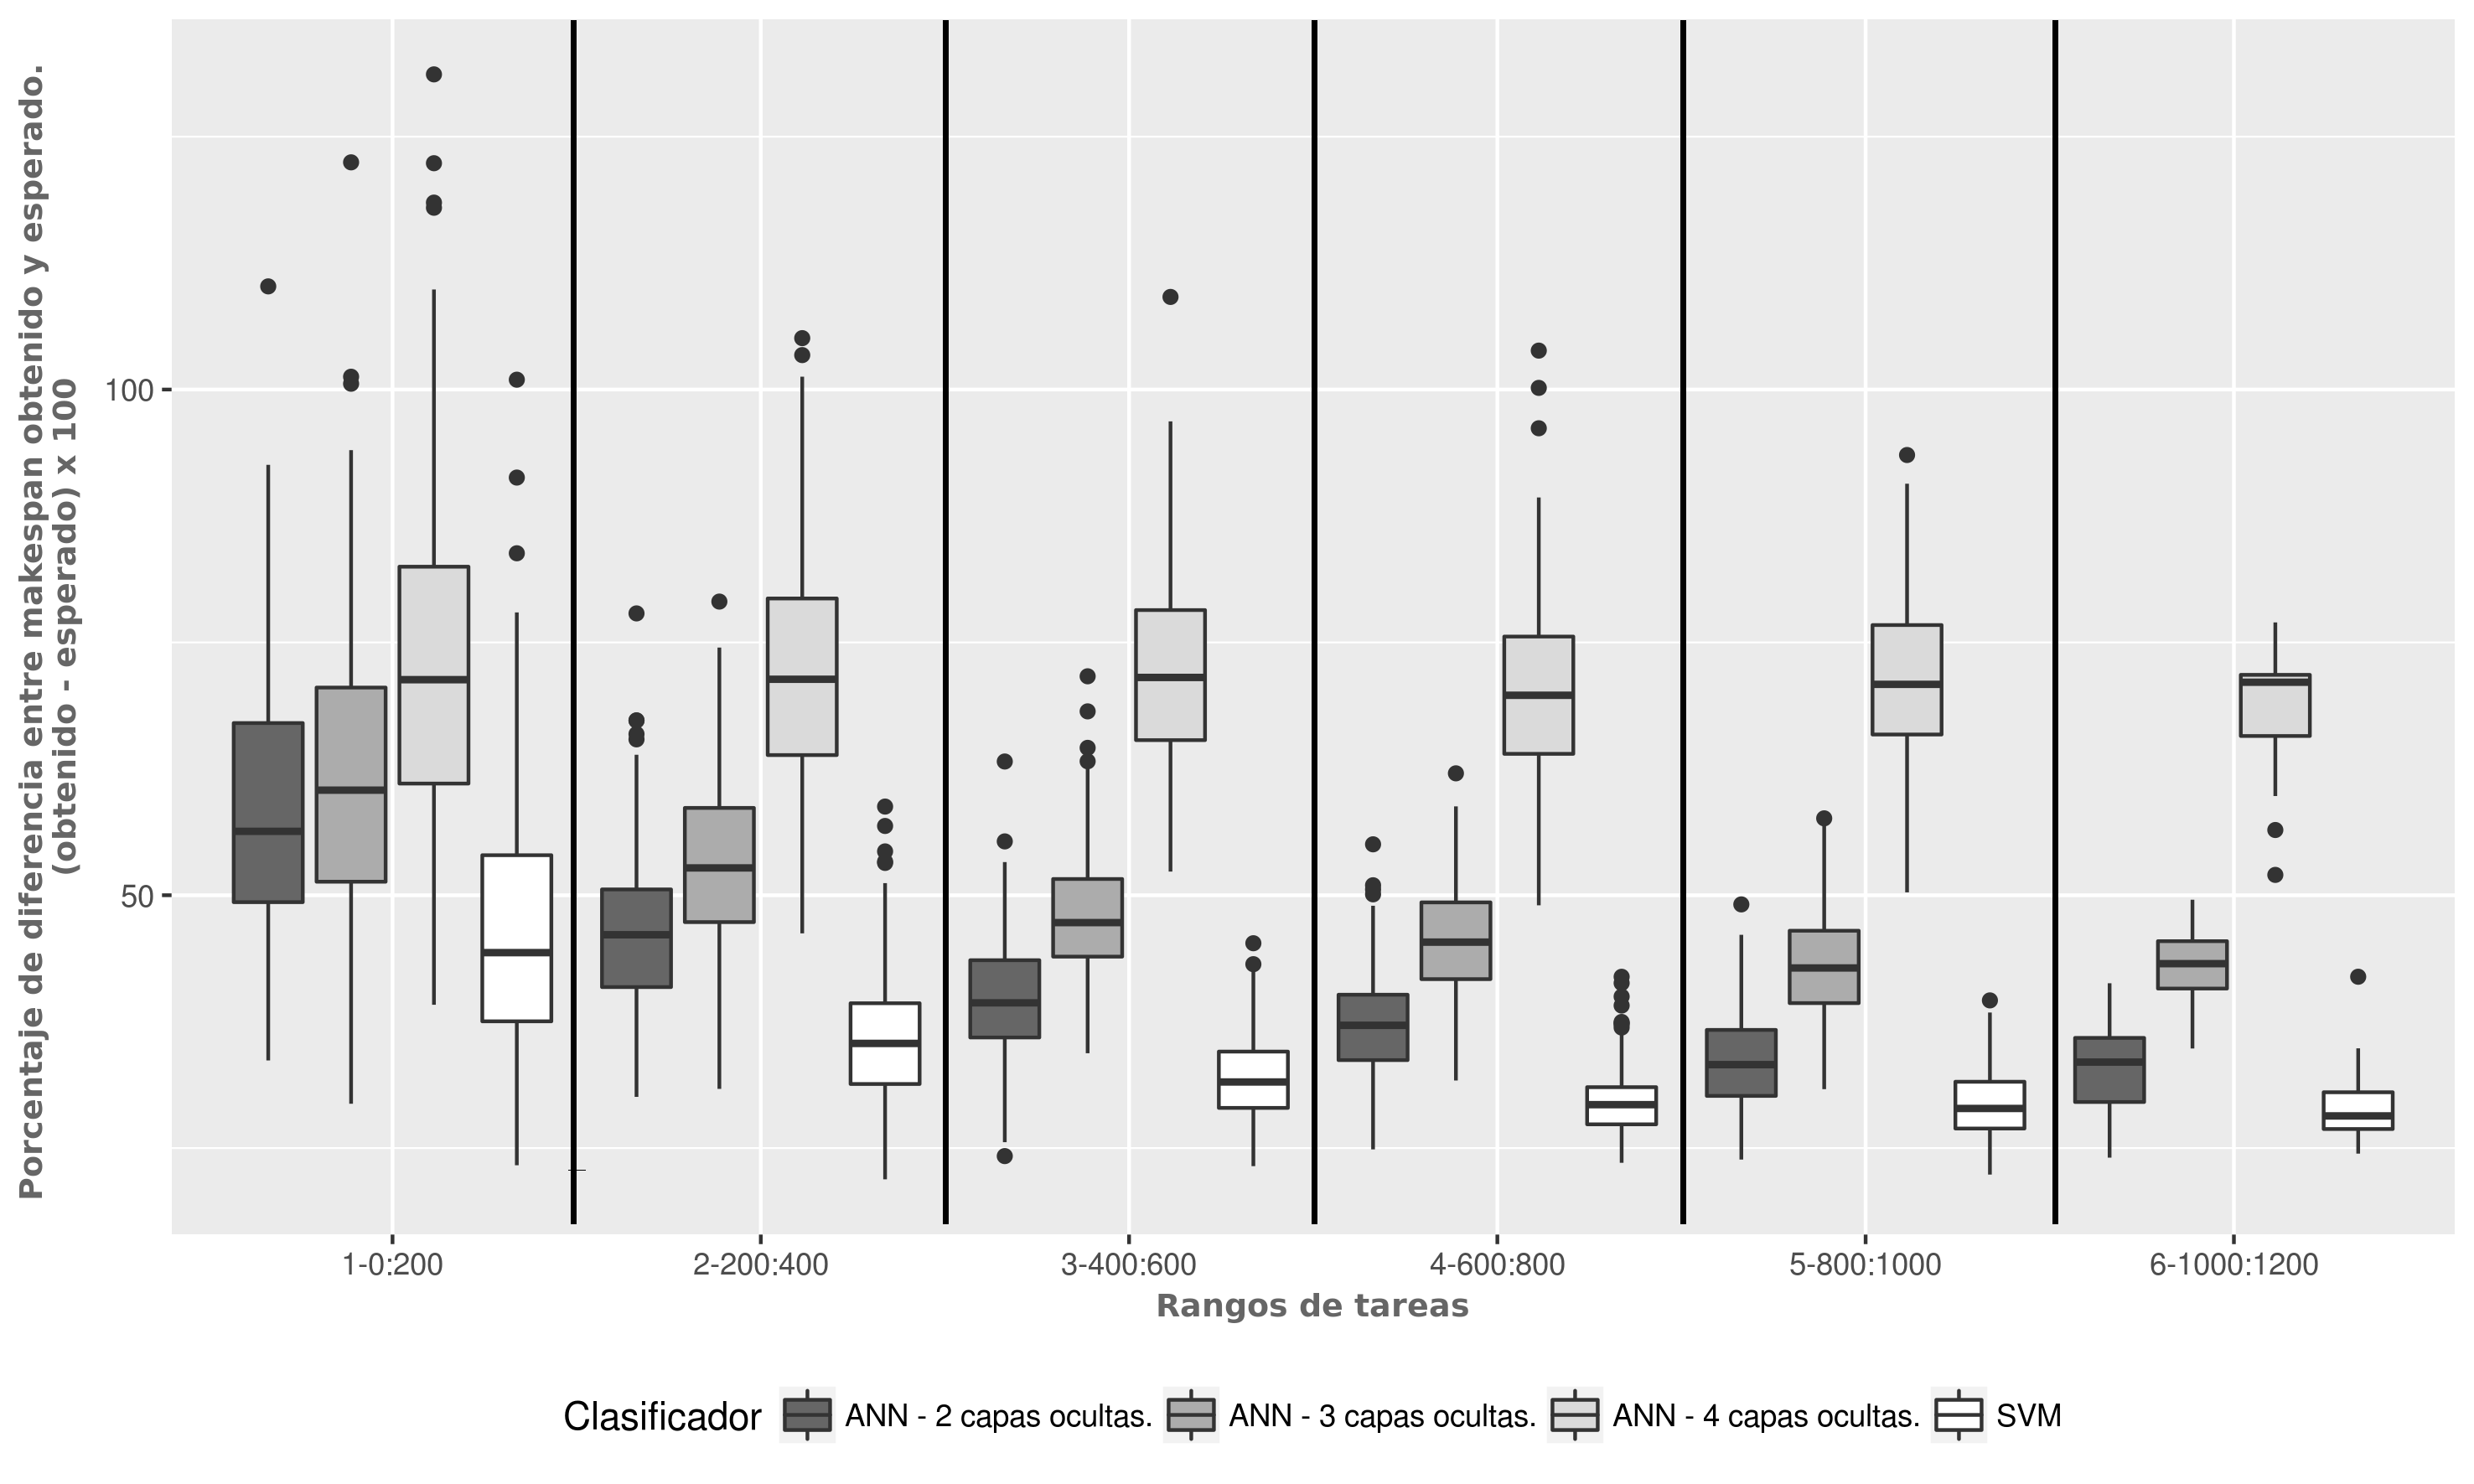
\includegraphics[width=\columnwidth]{imagenes/comparacion_anns_relu_2.png}
  \caption{Comparación de  la diferencia porcentual  de los resultados de \textit{makespan} para redes neuronales con función de activación \textit{relu} y para SVM, con respecto al \textit{makespan} obtenido por el algoritmo Min-Min.
Se comparan redes neuronales de 2, 3 y 4 capas ocultas.}
  \label{fig:relu234}
\end{figure}

\paragraph{}La Figura \ref{fig:identity234} muestra los resultados para las redes neuronales utilizando la función de activación \textit{identity}.
En este caso los resultados para las redes neuronales son más próximos a los valores esperados dados por el algoritmo Min-Min que los resultados dados por SVM.
Ya desde tareas de dimensión $ 200 \times 16$ se comienzan a observar mejoras en el \textit{makespan}, siendo aún más evidentes para instancias del problema de dimensión mayor.
Nuevamente se observa que los resultados más próximos al \textit{makespan} esperado están dados por la red neuronal con dos capas ocultas. 

\newpage % orphaned line.

\paragraph{}En la Figura \ref{fig:tanh234} se observan los resultados para las redes neuronales utilizando la función de activación \textit{tanh}.
En este caso, la red neuronal con dos capas ocultas mejora los resultados obtenidos a partir de instancias del problema de dimensión $ 400 \times 16$ en adelante. 

\paragraph{} En los casos presentados en las Figuras \ref{fig:relu234}, \ref{fig:identity234} y \ref{fig:tanh234}, los mejores resultados de las redes neuronales se encontraron para aquellas de solo dos capas ocultas. Fue profundizado el estudio de las redes neuronales con solo dos capas ocultas, de cara a entender mejor la naturaleza de las soluciones generadas. 

\textsc{\begin{figure}[H]
  \centering
  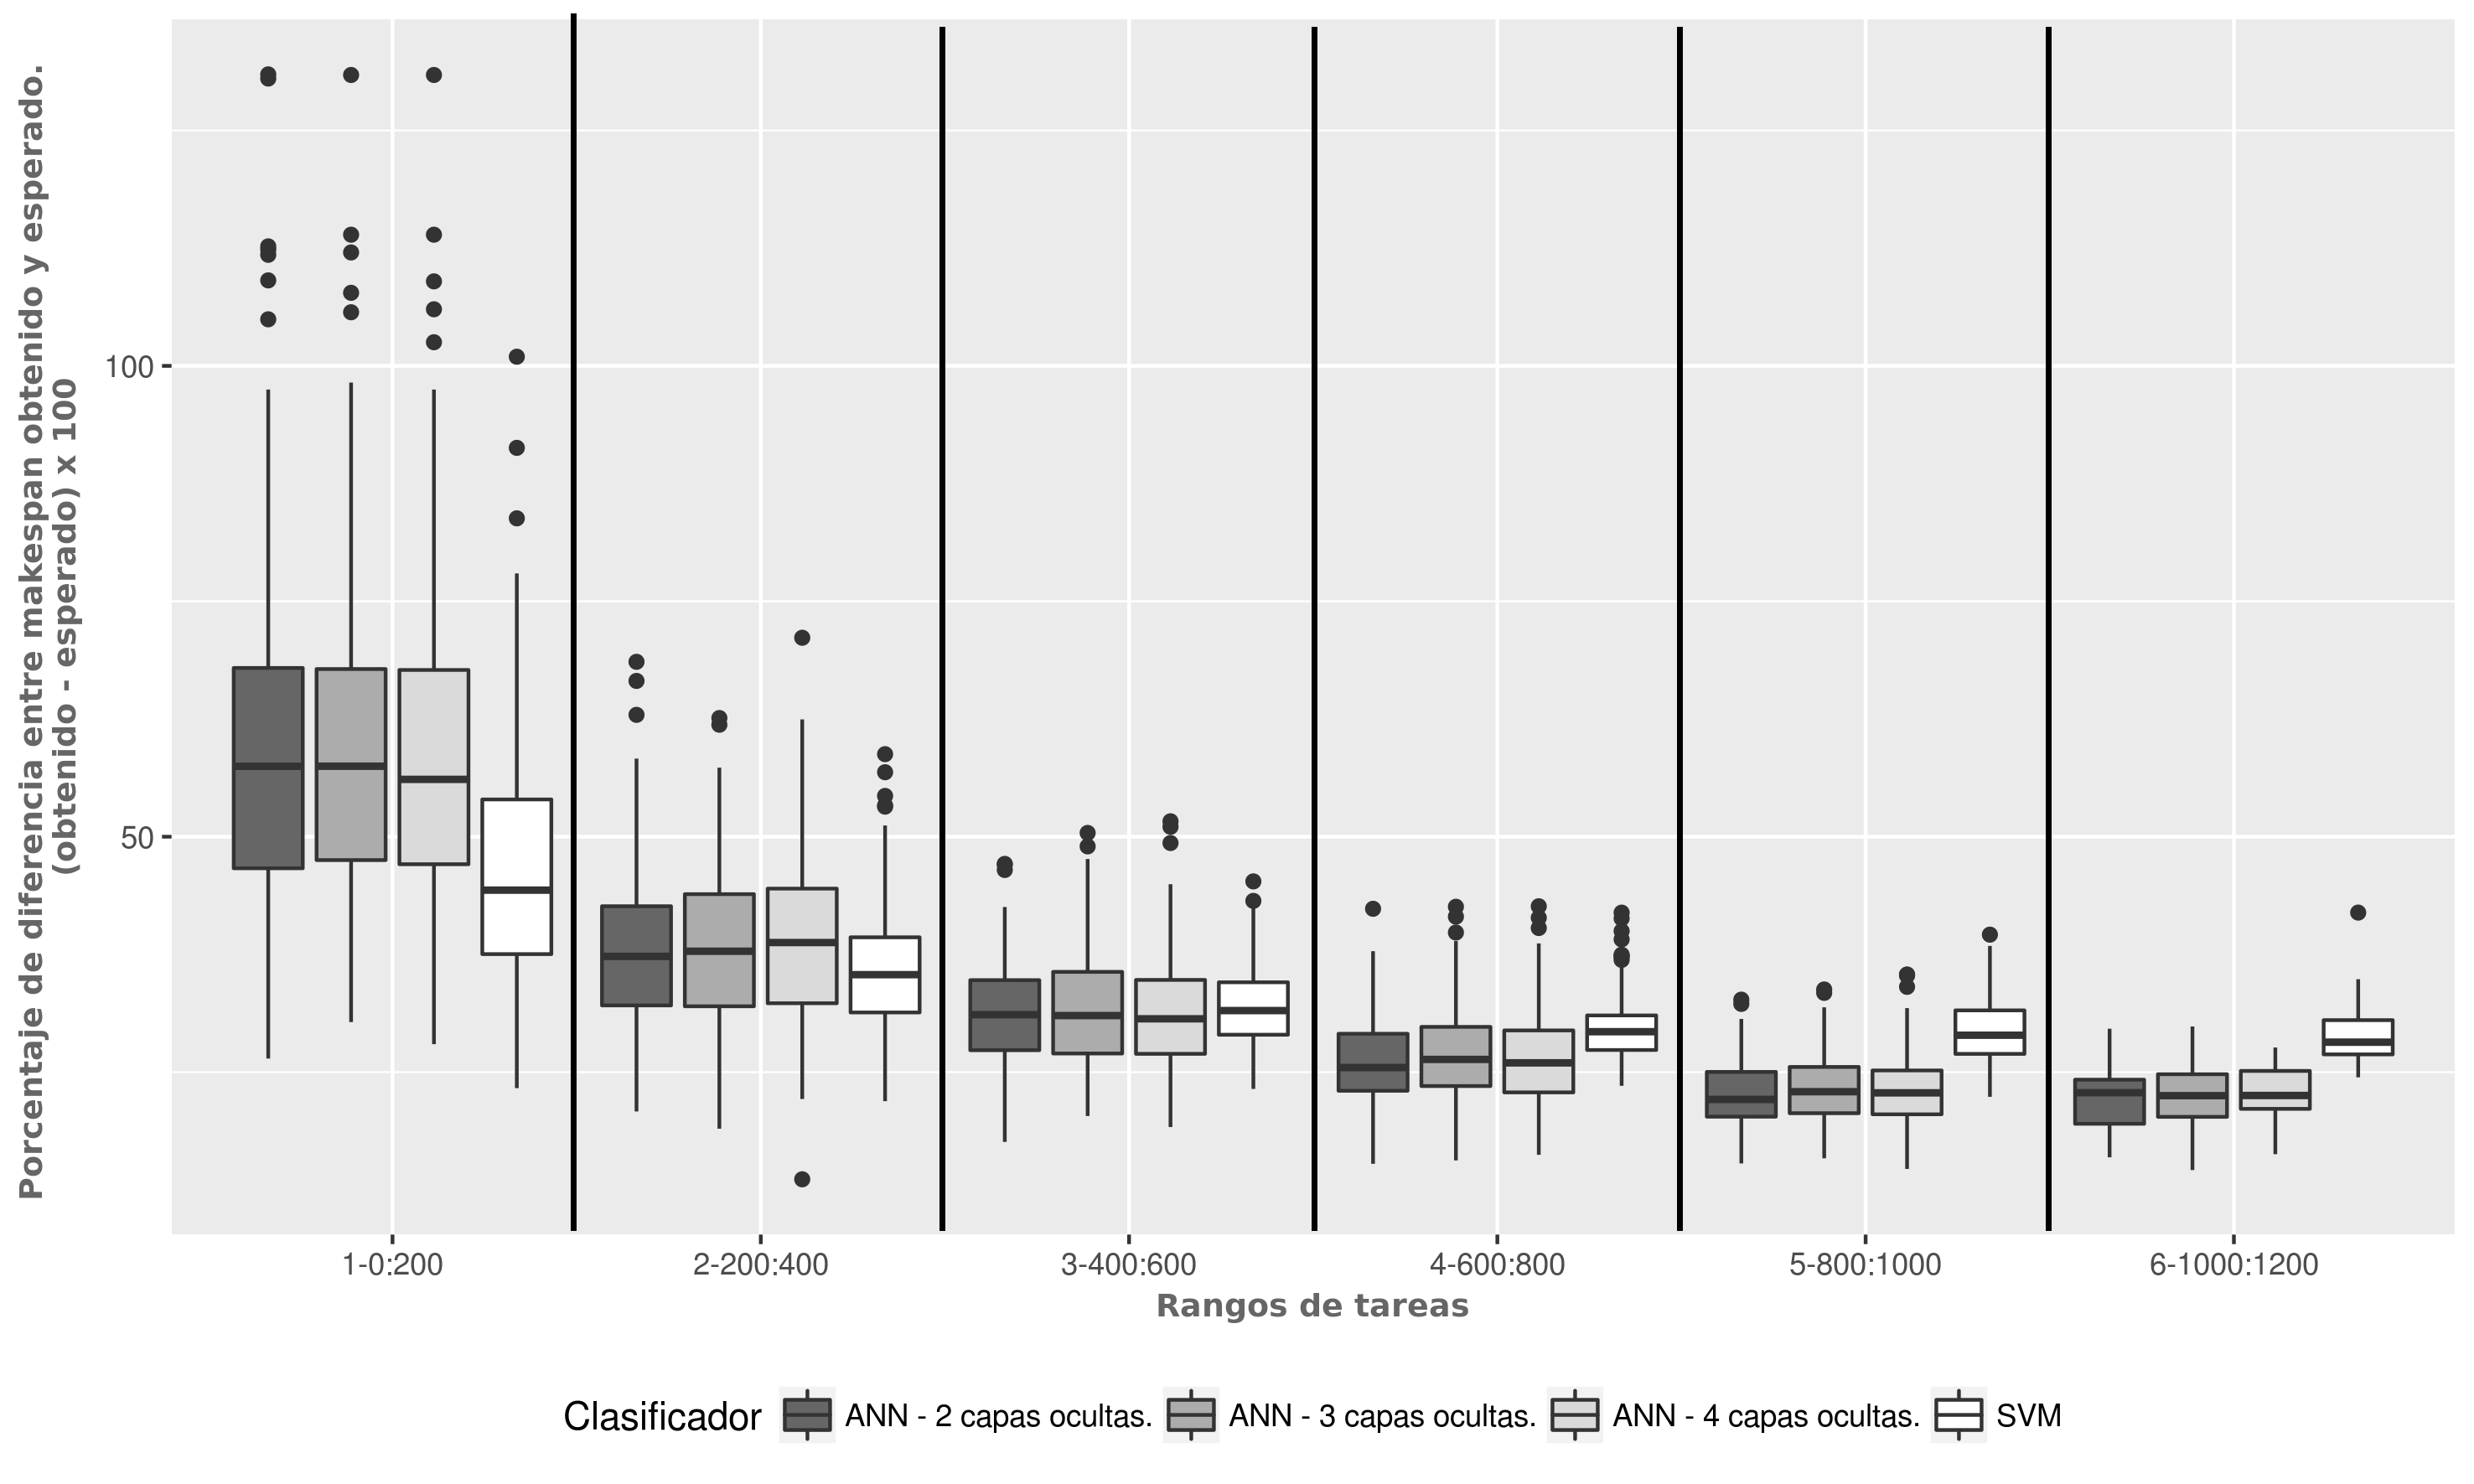
\includegraphics[width=\columnwidth]{imagenes/comparacion_anns_identity_2.png}
  \caption{Comparación de  la diferencia porcentual  de los resultados de \textit{makespan} para redes neuronales con función de activación \textit{identity} y para SVM, con respecto al \textit{makespan} obtenido por el algoritmo Min-Min. Se comparan redes neuronales de 2, 3 y 4 capas. Así también se muestran los resultados obtenidos con el algoritmo de SVM.}
  \label{fig:identity234}
\end{figure}}

\newpage % orphaned line.

\textsc{\begin{figure}[H]
  \centering
  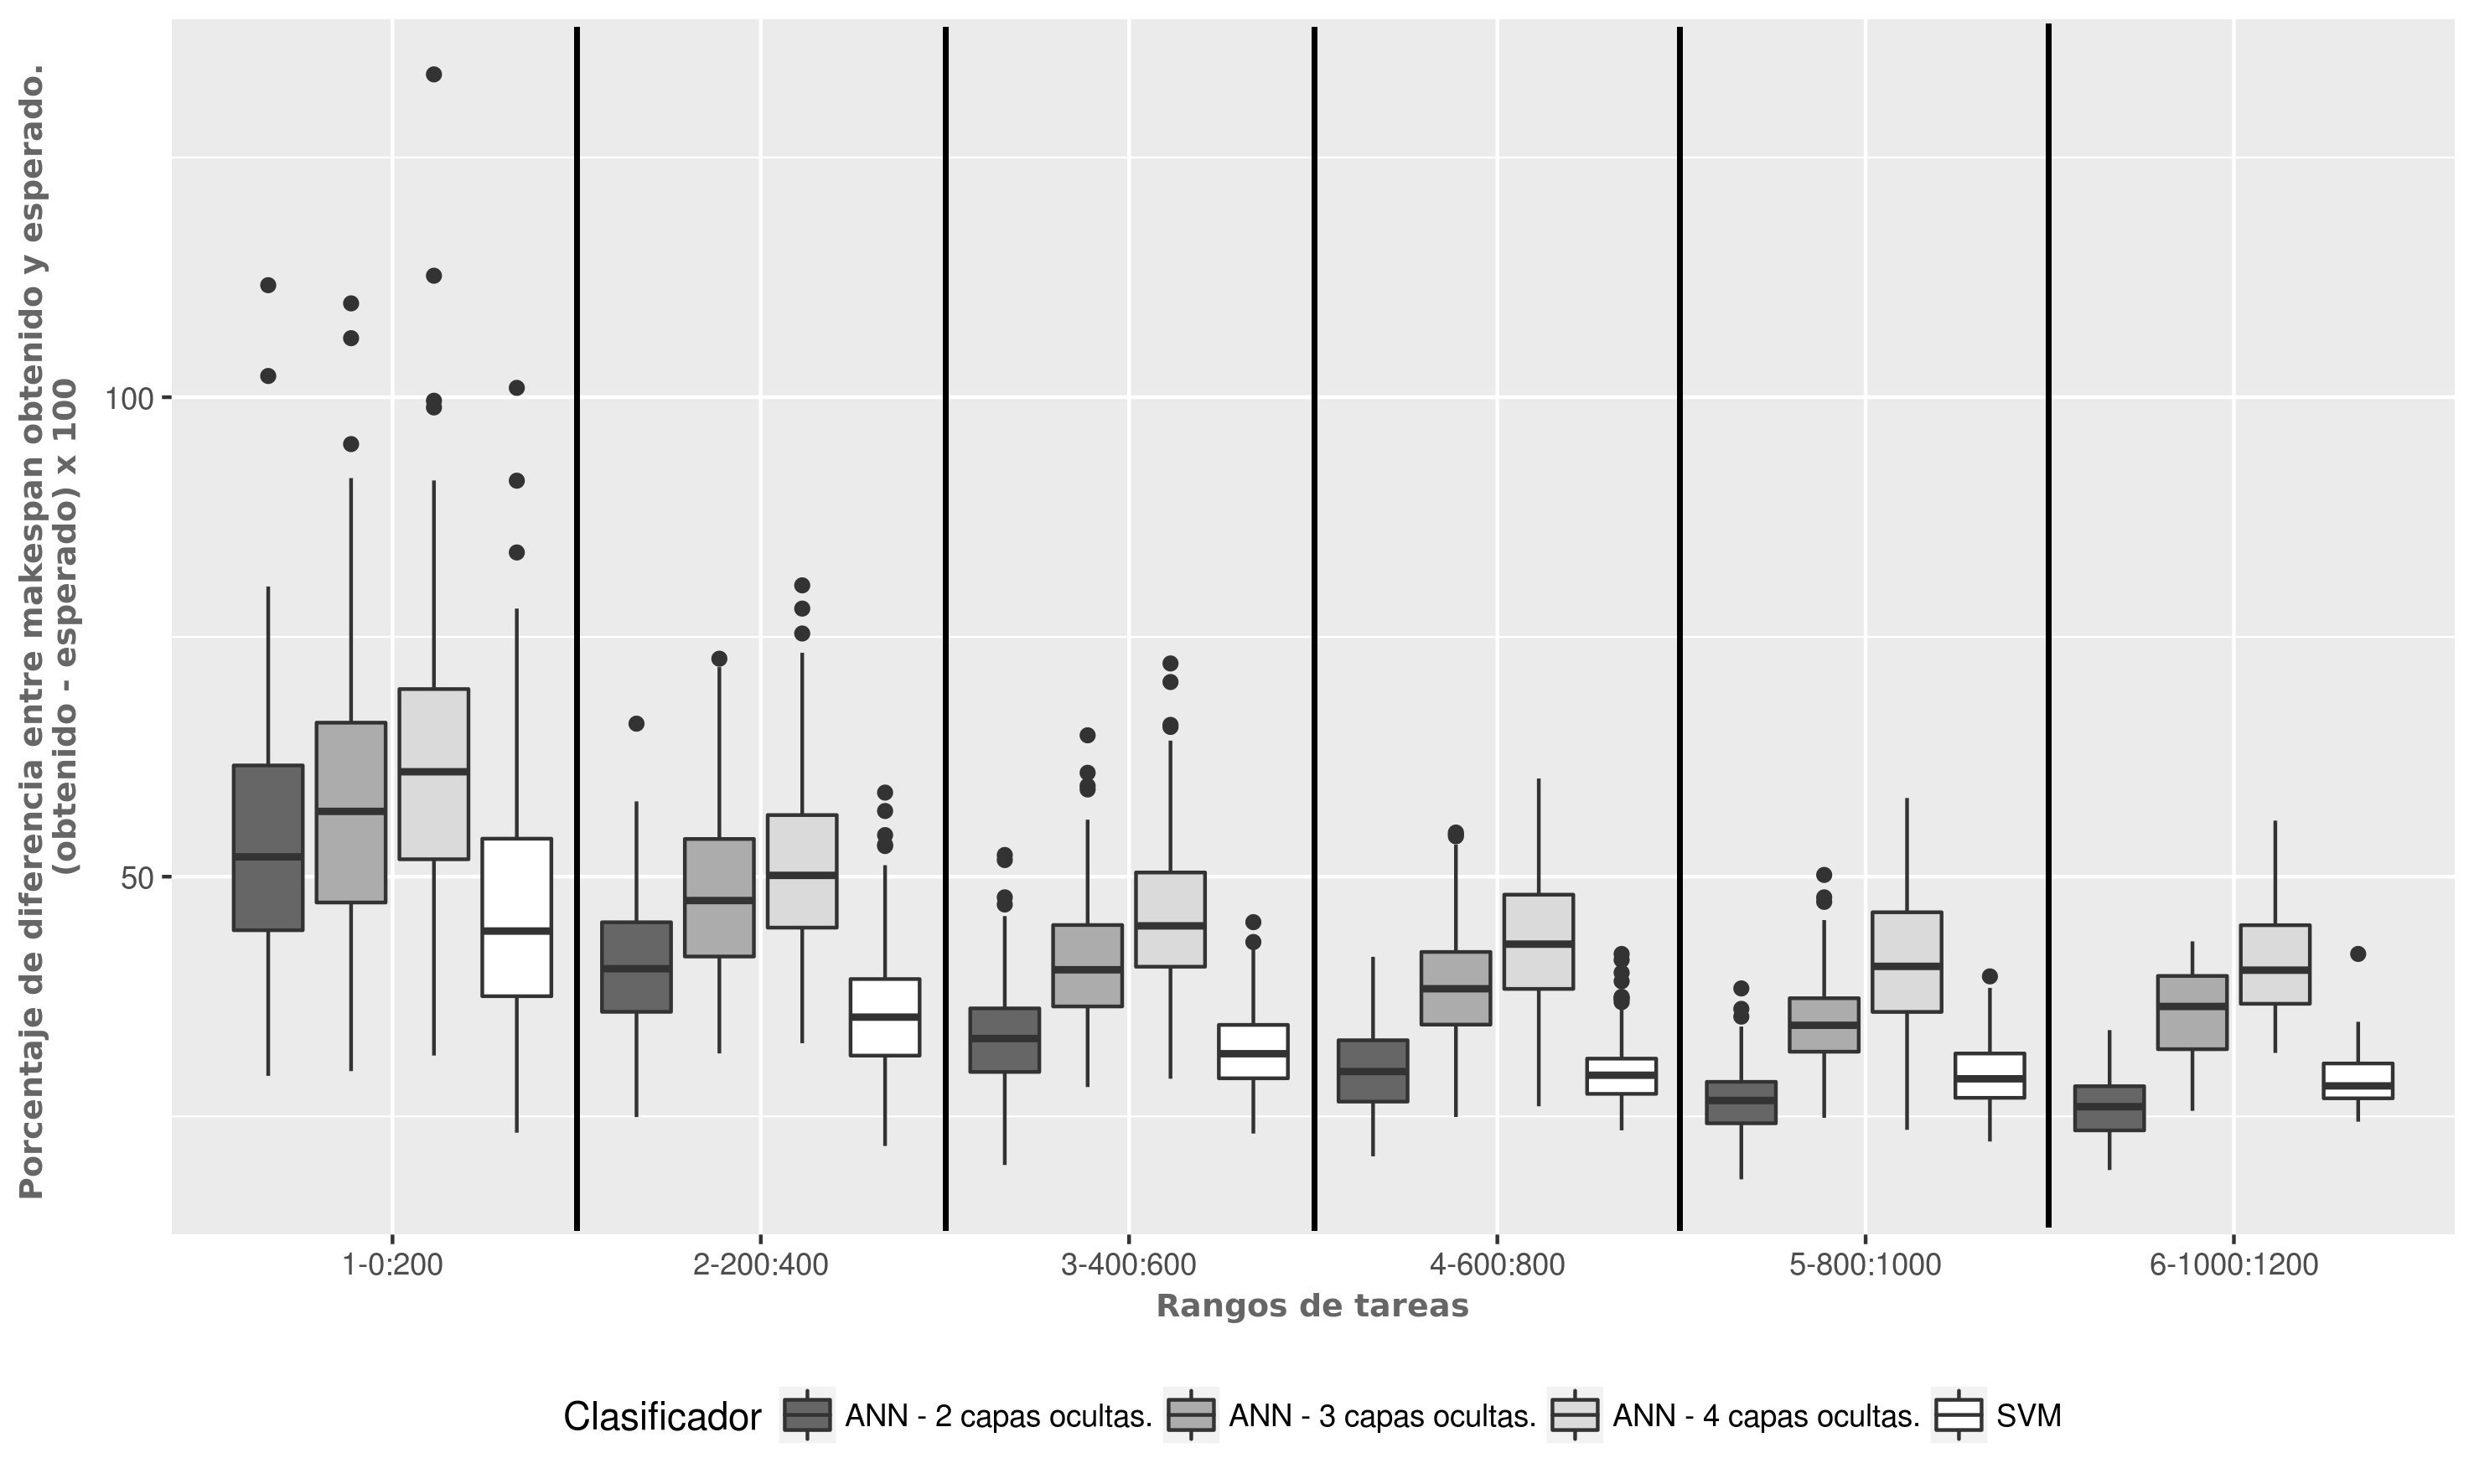
\includegraphics[width=\columnwidth]{imagenes/comparacion_anns_tanh_2.png}
  \caption{Comparación de  la diferencia porcentual  de los resultados de \textit{makespan} para redes neuronales con función de activación \textit{tanh} y para SVM, con respecto al \textit{makespan} obtenido por el algoritmo Min-Min.
Se comparan redes neuronales de 2, 3 y 4 capas.
Así también se muestran los resultados obtenidos con el algoritmo de SVM.}
  \label{fig:tanh234}
\end{figure}}

\newpage % orphaned line.

\section{Red neuronal con activación \textit{relu} de dos capas ocultas}

La Figura \ref{fig:relu_makespan} muestra la diferencia porcentual de \textit{makespan} entre la red neuronal de dos capas ocultas con función de activación \textit{relu} y la SVM con respecto al \textit{makespan} esperado.
Como ya se observó, la SVM muestra valores más próximos a los valores esperados que la red neuronal. 

\paragraph{} Por otro lado, la Figura \ref{fig:relu_accuracy} muestra la precisión de la clasificación para ambos clasificadores.
Se observa que la precisión en la clasificación aumenta a medida que la dimensión de las instancias de prueba aumenta, tanto para la red neuronal como para la SVM. 

\begin{figure}[H]
  \centering
  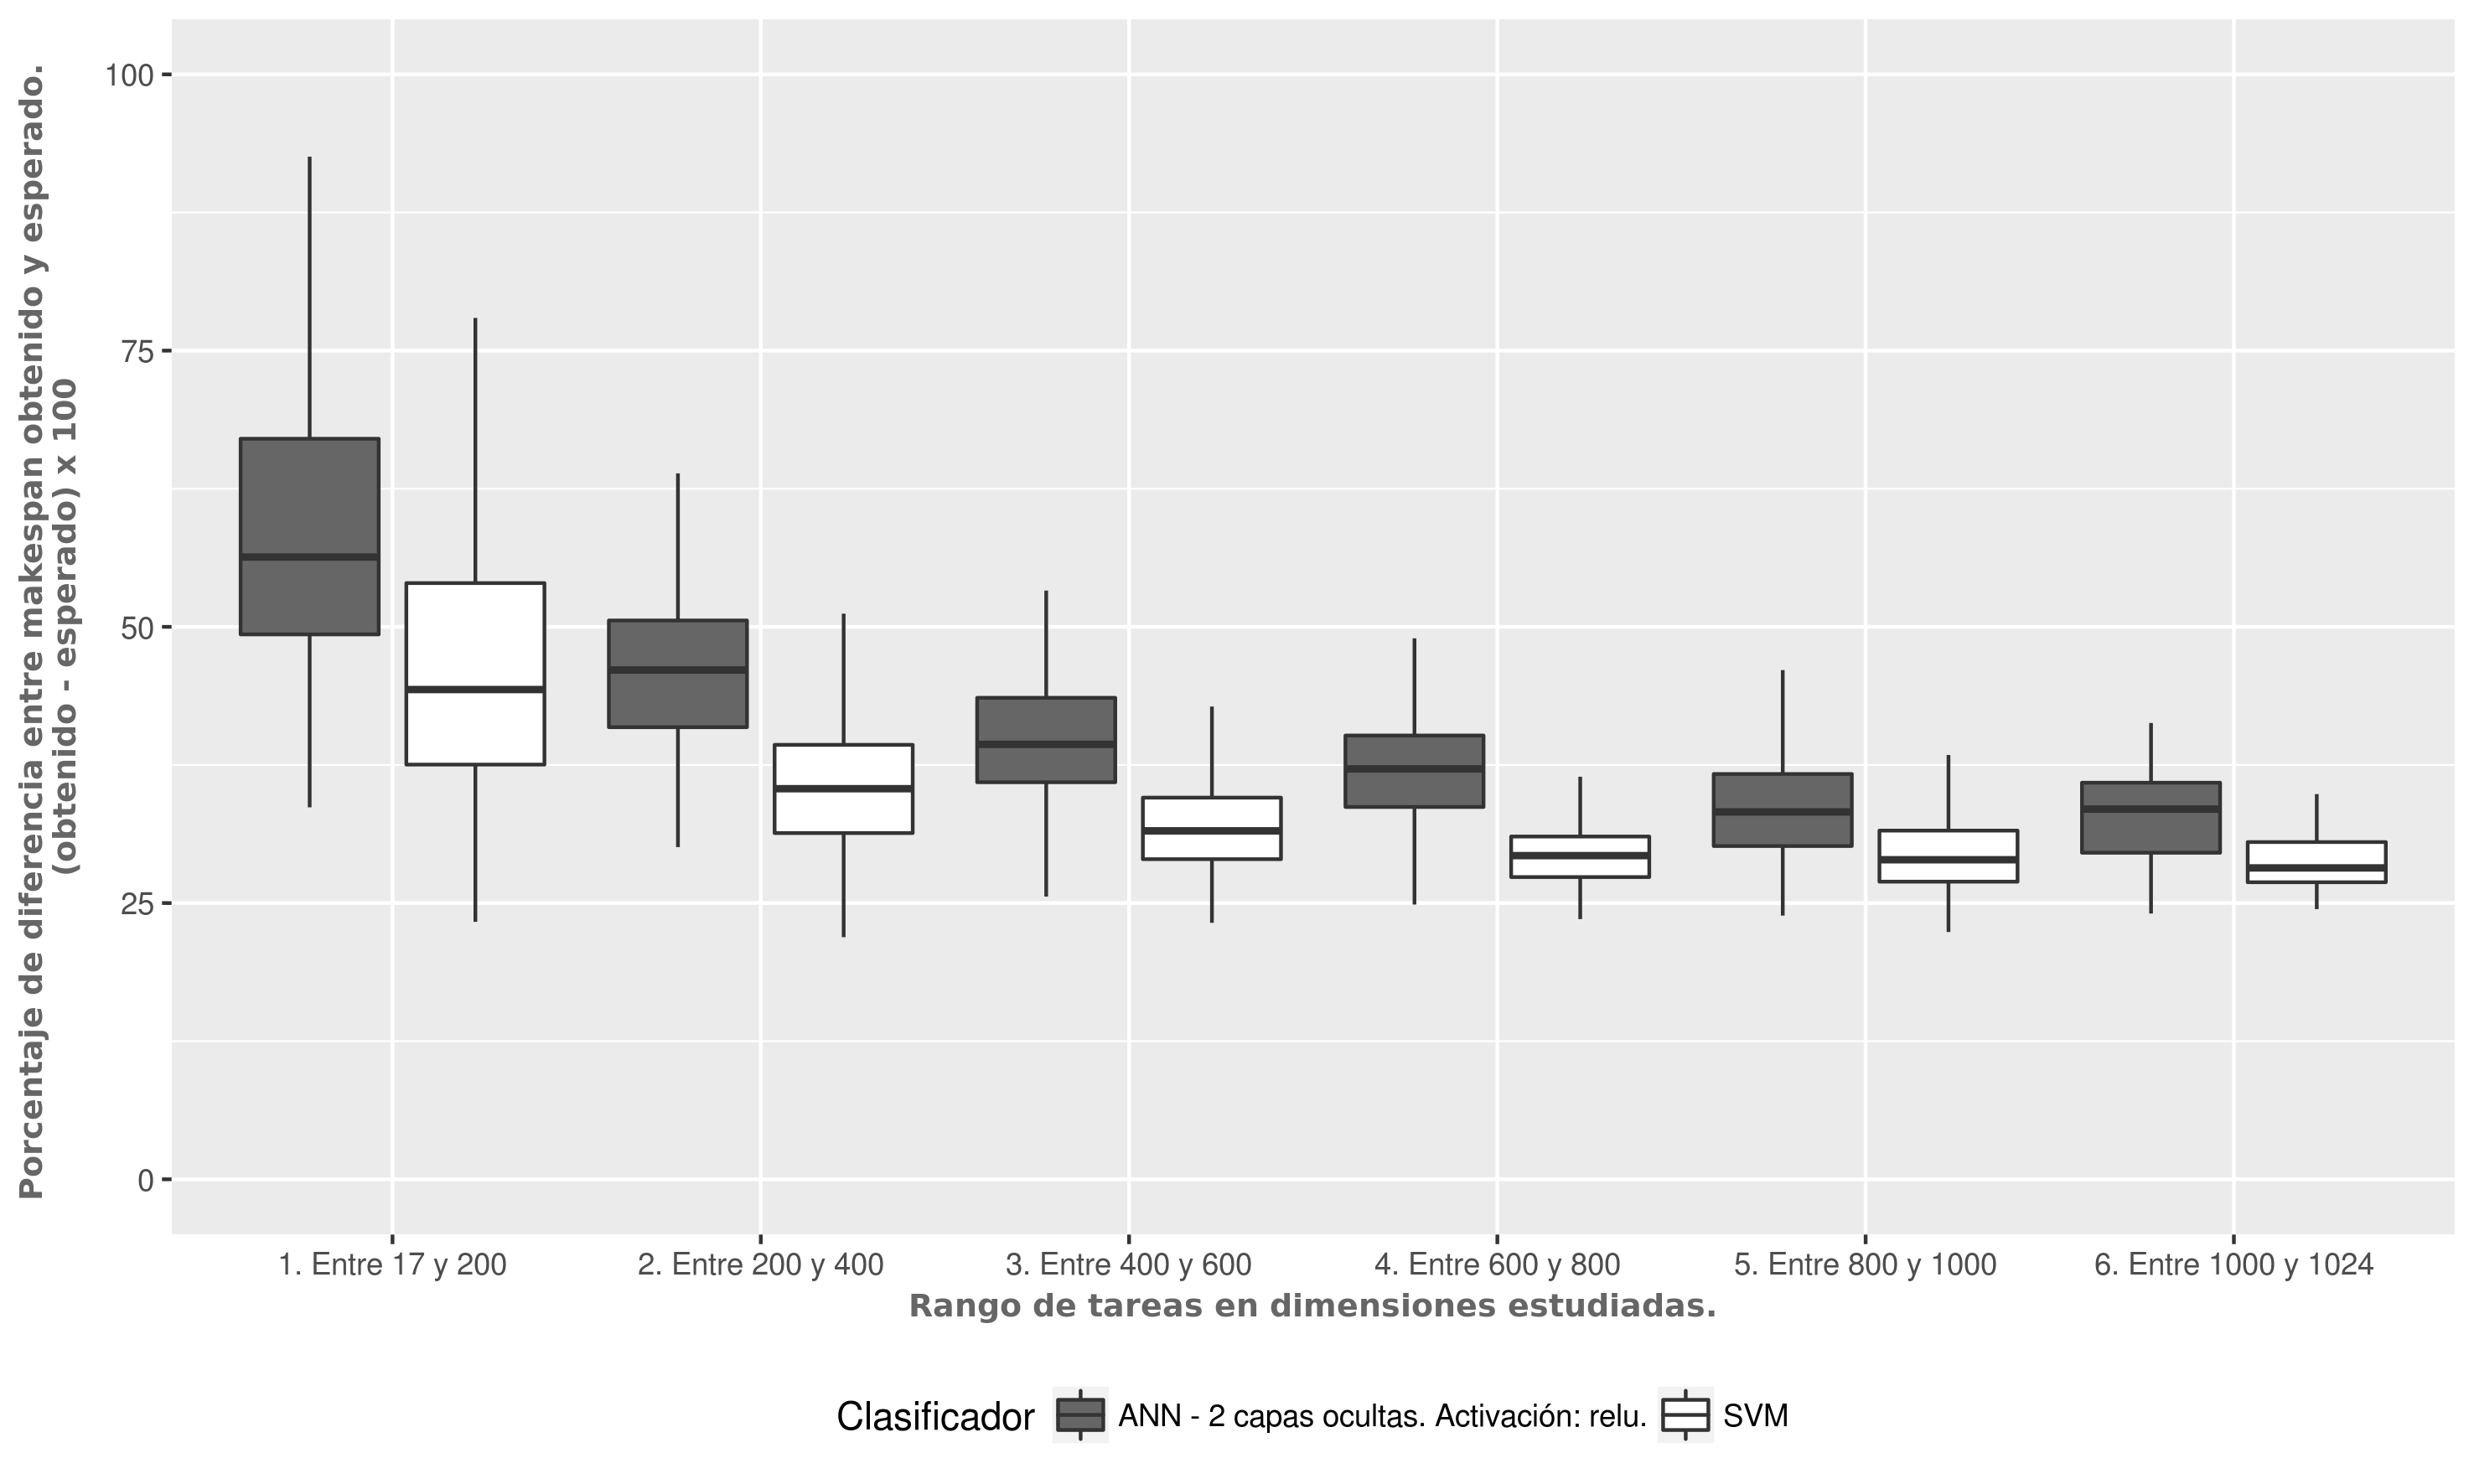
\includegraphics[width=\columnwidth]{imagenes/relu/2_medianas_diferenciasann_2_capas_ocultas_relu.png}
  \caption{Comparación de la diferencia porcentual de \textit{makespan} para la red neuronal con activación \textit{relu}, de dos capas ocultas con respecto a los valores esperados obtenidos con el algoritmo Min-Min.
Así también se muestran los resultados obtenidos para la SVM.
Los resultados se muestran divididos en rangos de dimensión desde $ 17 \times 16$ a $ 1024 \times 16$.}
  \label{fig:relu_makespan}
\end{figure}

\newpage % orphaned line.

\paragraph{}La precisión de la red neuronal es levemente mayor que la precisión de la SVM.
Esto, en comparación con la diferencia de \textit{makespan} de la Figura \ref{fig:relu_makespan}, es de interés dado que, si bien la precisión de la red neuronal es levemente mejor, la SVM genera mejores resultados en términos de \textit{makespan}.
Este escenario también fue identificado para las demás redes neuronales en las cuales se profundizaron los estudios. 

\paragraph{} Para poder explicar lo antedicho, se calculó el porcentaje de selección de mejores máquinas para ambos clasificadores, como se menciona en la Sección \ref{chapter-implementacion:clasificacion}.
La Figura \ref{fig:relu_maquinas_mejores} muestra dicha métrica para ambos clasificadores.
Se puede observar que SVM elige más máquinas con menor tiempo de ejecución que la red neuronal, cuando  se seleccionan máquinas diferentes a las esperadas. 

\begin{figure}[H]
  \centering
  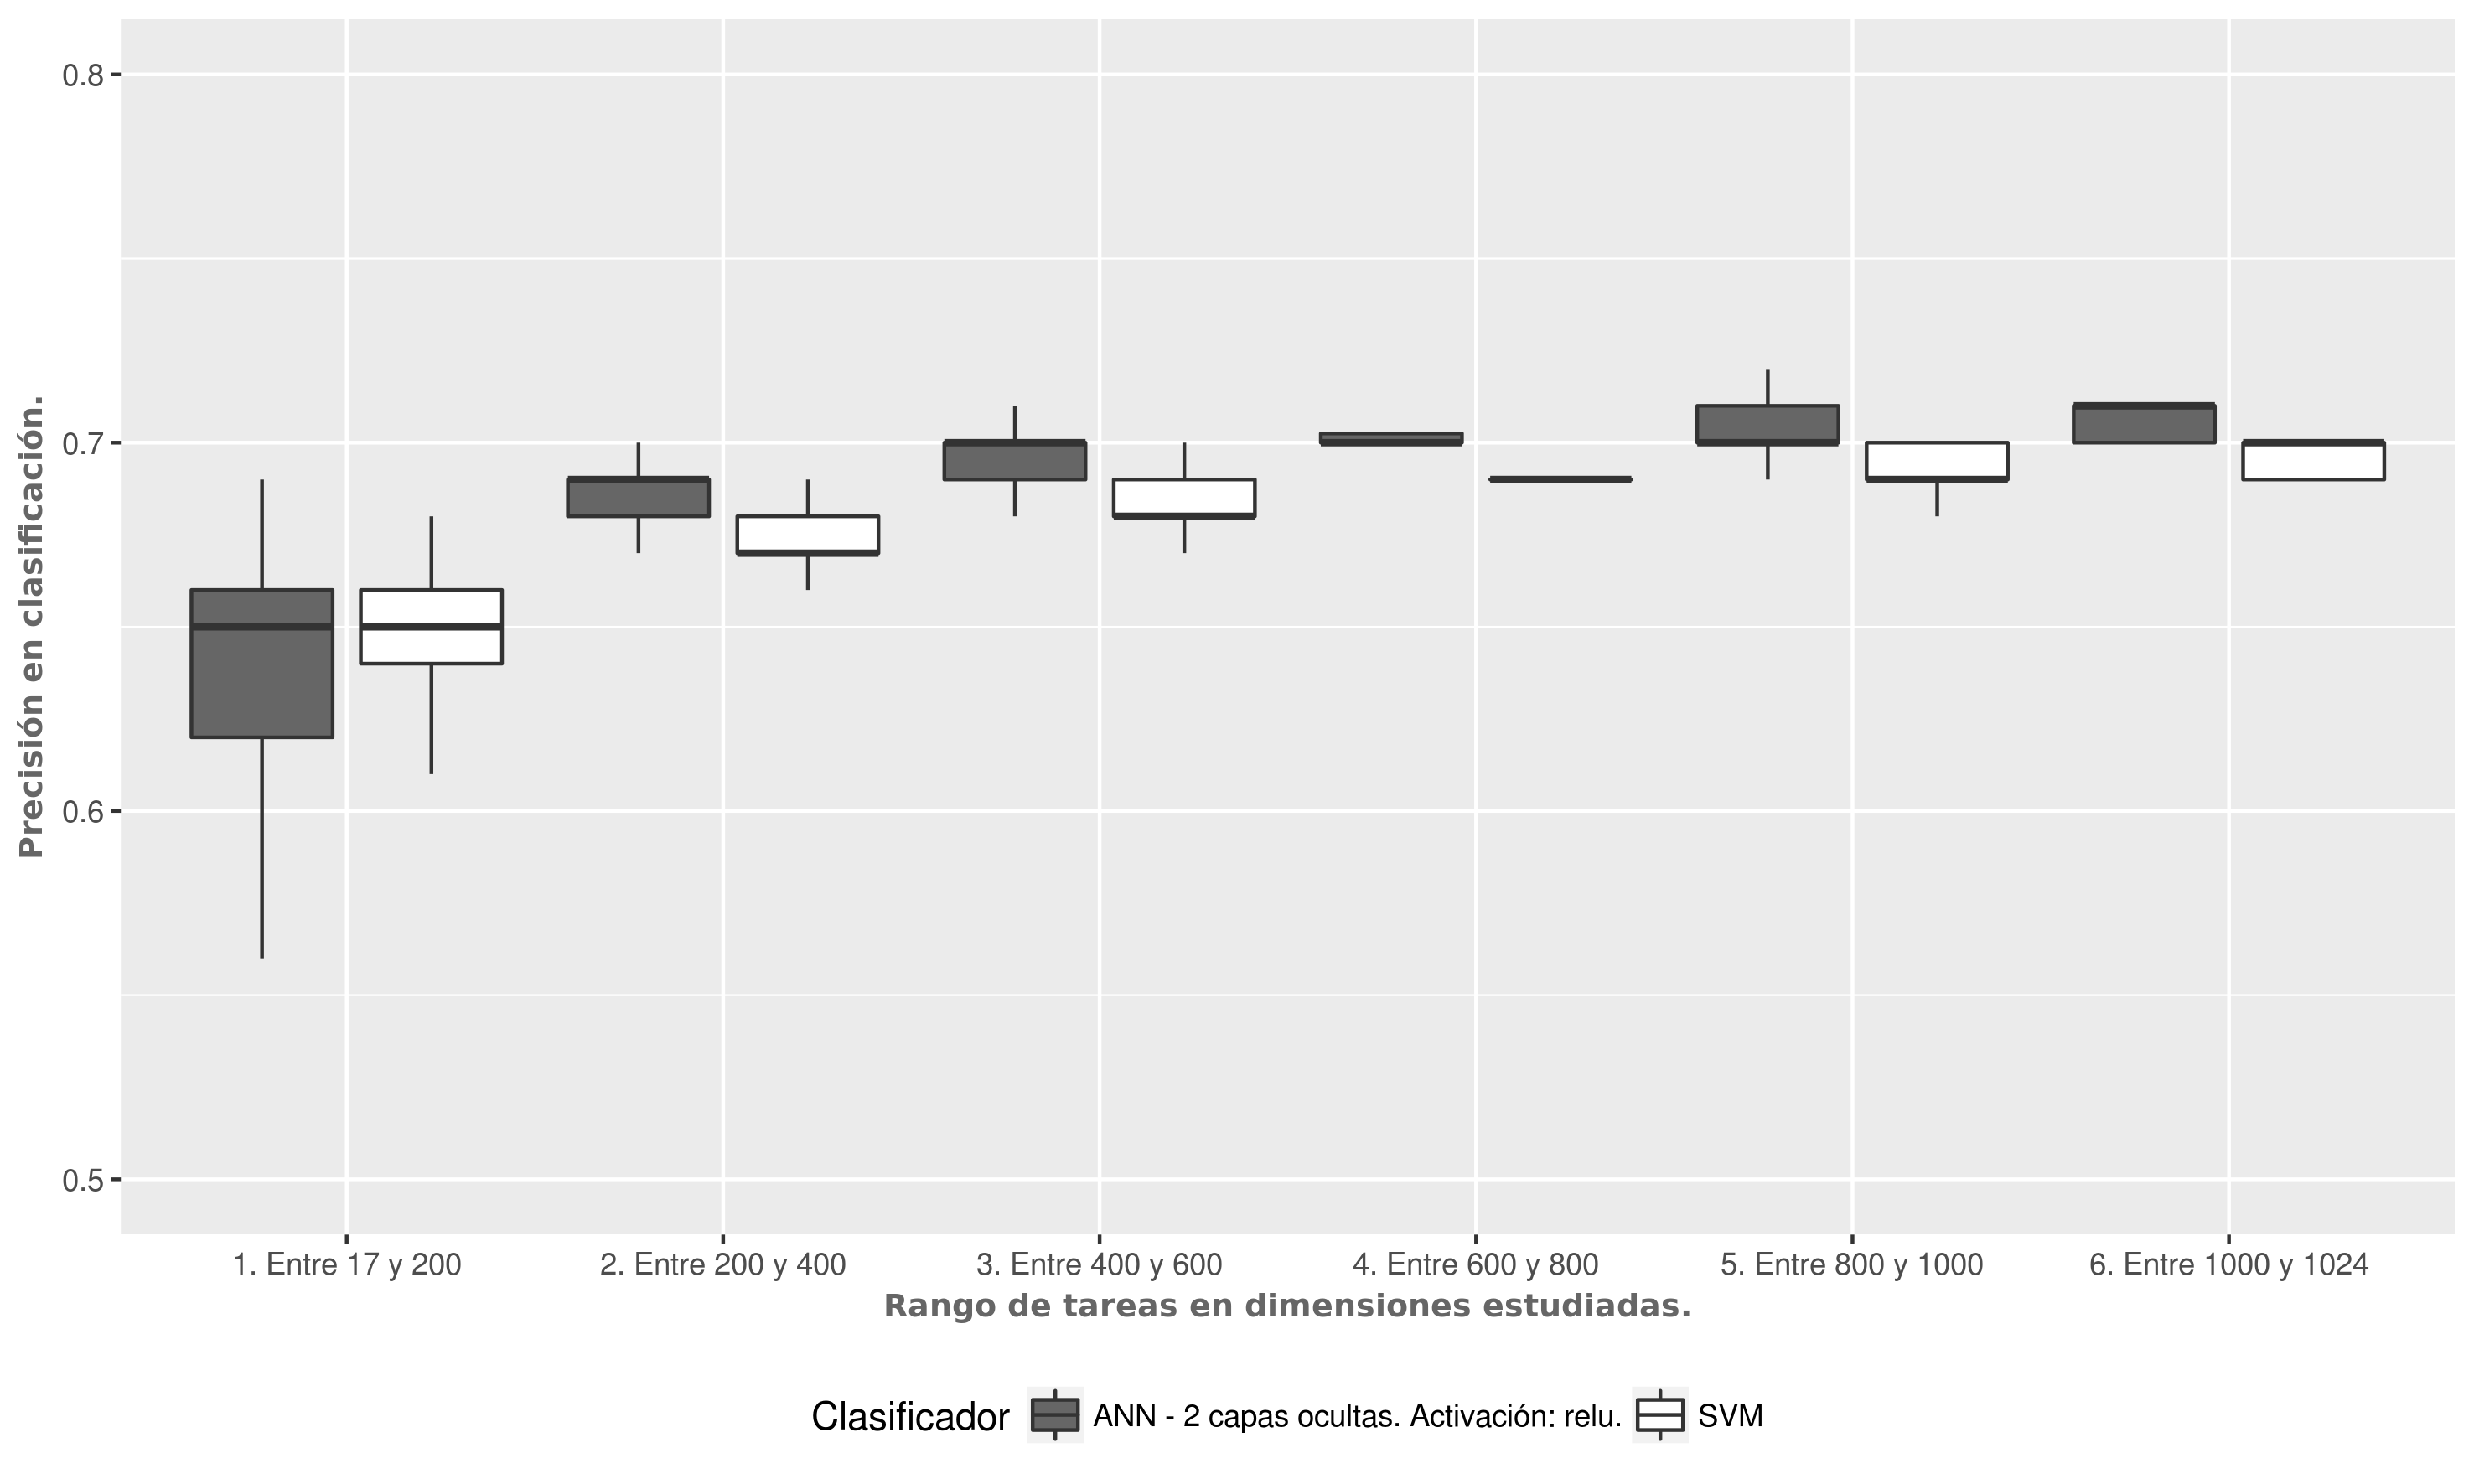
\includegraphics[width=\columnwidth]{imagenes/relu/3_accuracy_ann_2_capas_ocultas_relu.png}
  \caption{Precisión en clasificación para la red neuronal con función de activación \textit{relu} de dos capas ocultas y para la SVM.
Los resultados se muestran divididos en rangos de dimensión desde $ 17 \times 16$ a $ 1024 \times 16$.}
  \label{fig:relu_accuracy}
\end{figure}

\newpage % orphaned line.

\begin{figure}[H]
  \centering
  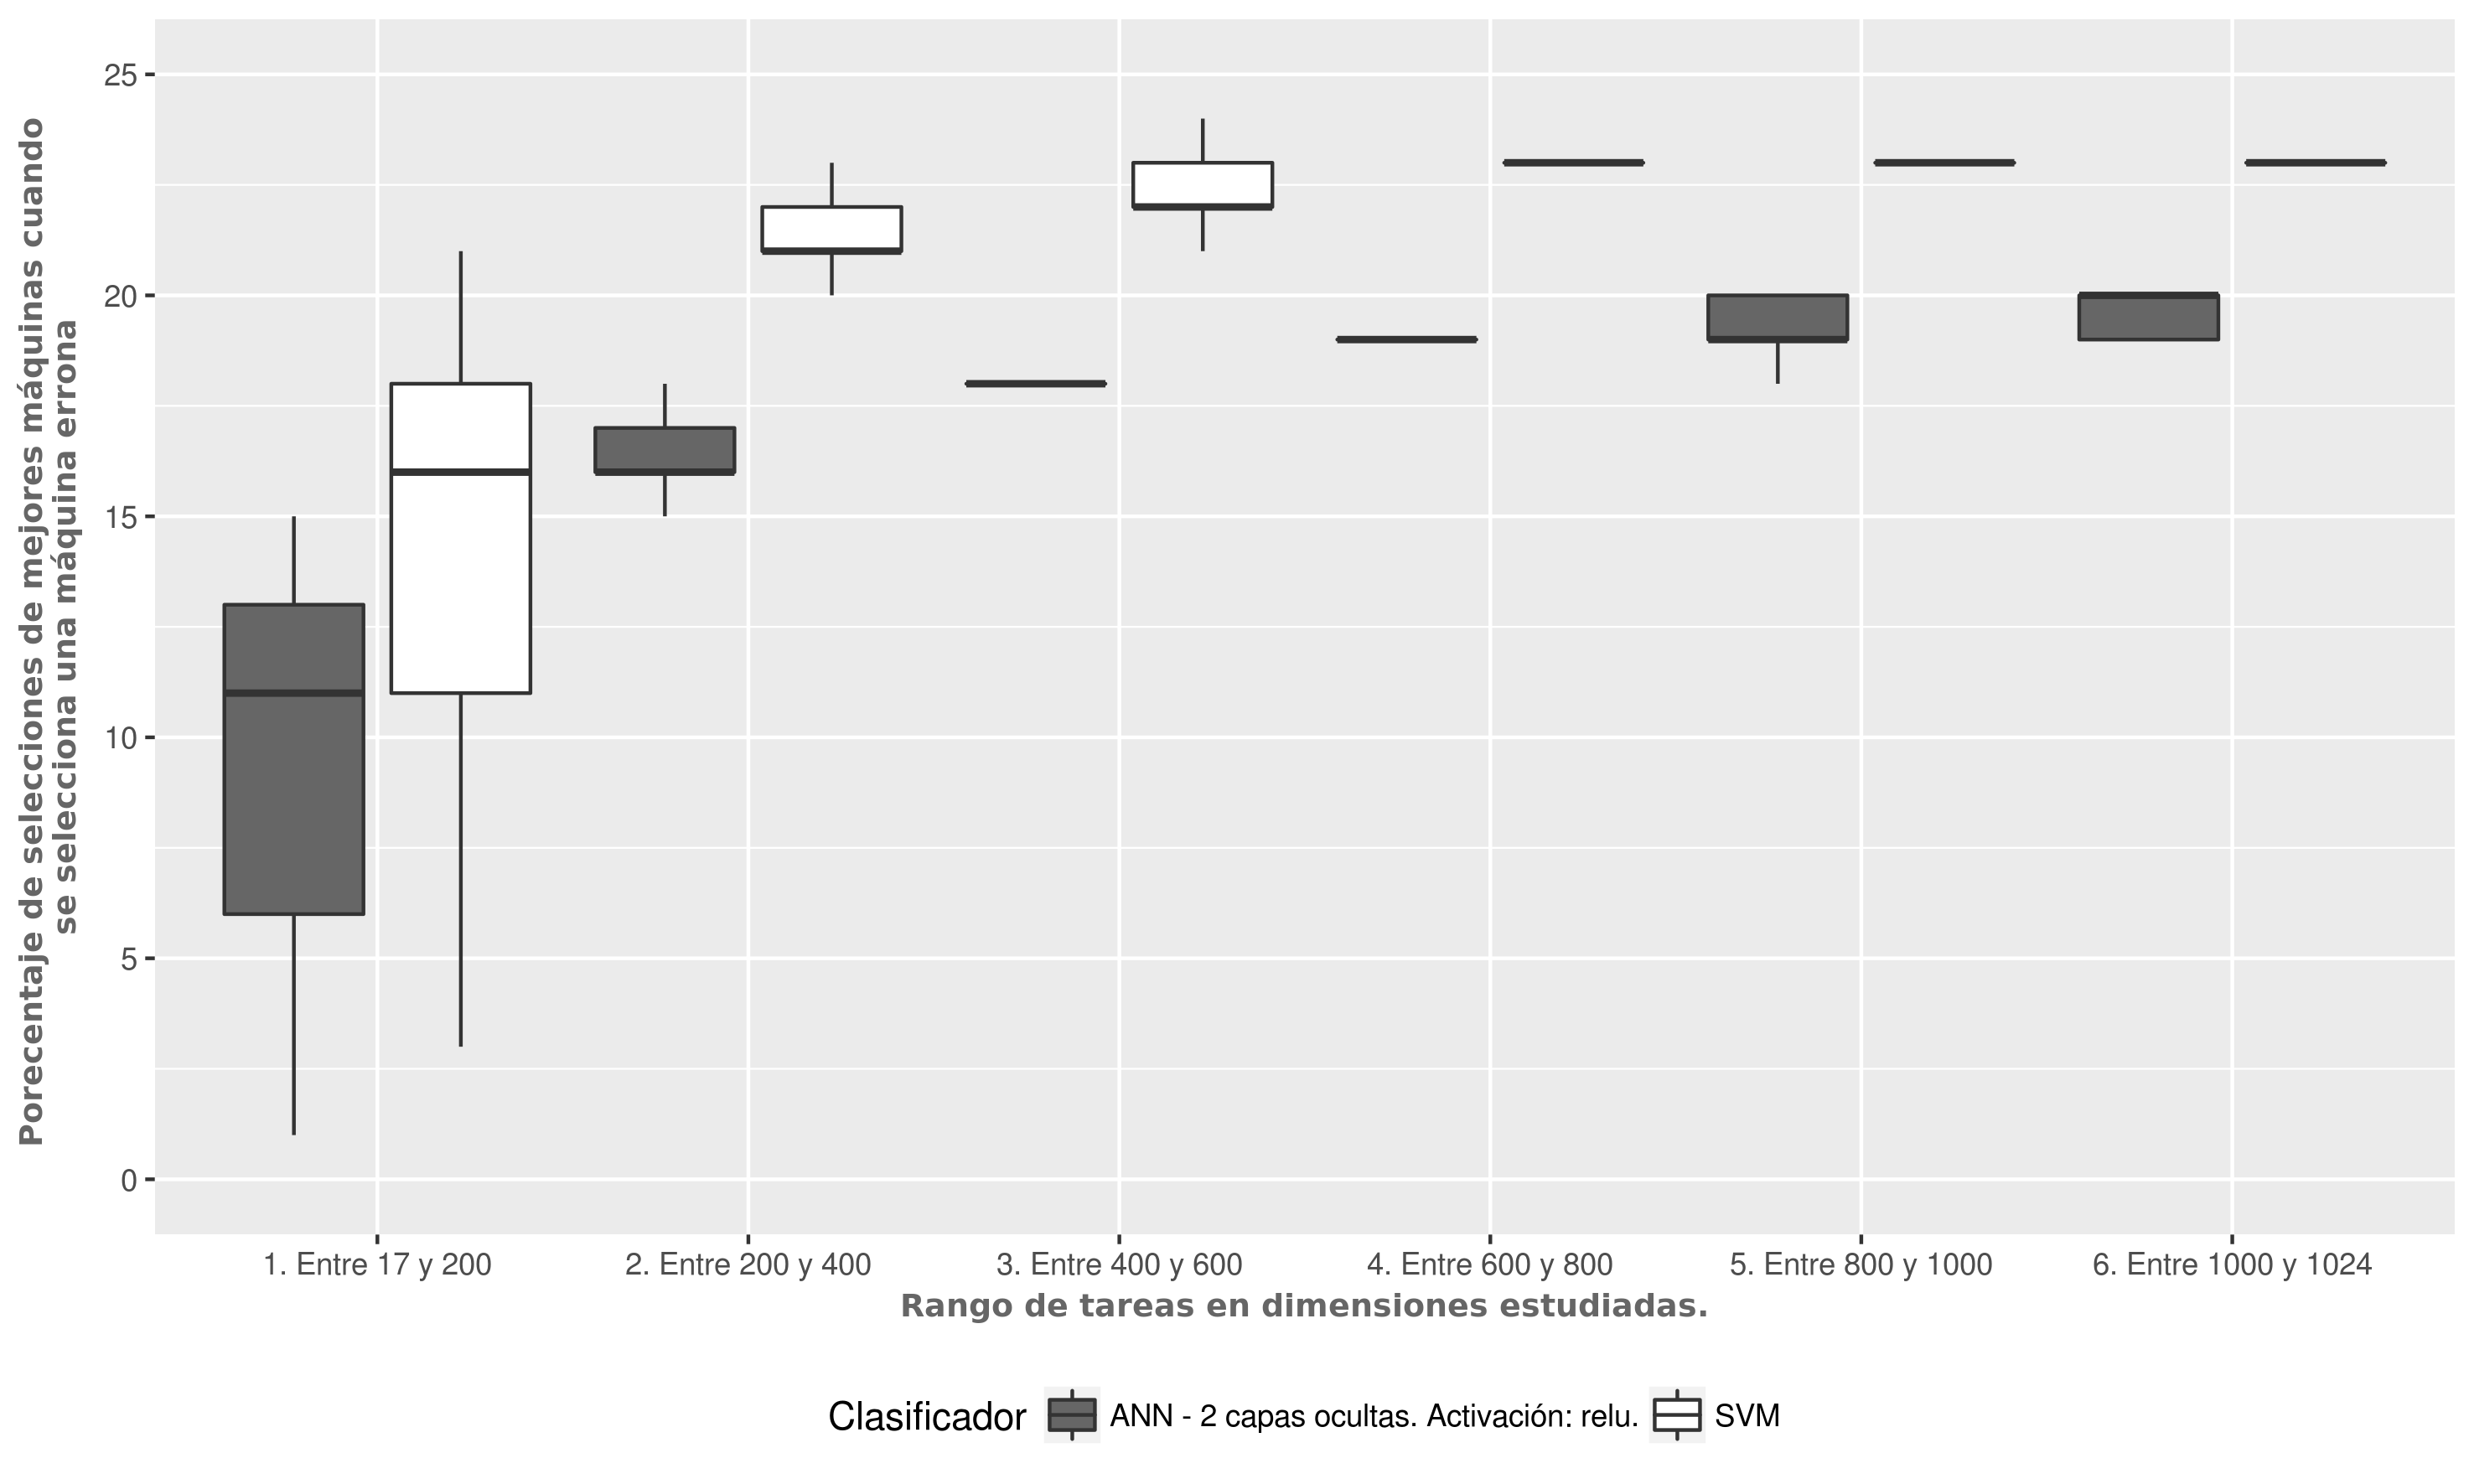
\includegraphics[width=\columnwidth]{imagenes/relu/4_porcentaje_maquinas_mejores_ann_2_capas_ocultas_relu.png}
  \caption{Porcentaje de selección de máquinas mejores frente a una selección diferente a la esperada para la red neuronal con activación \textit{relu} de dos capas ocultas y para la SVM.}
  \label{fig:relu_maquinas_mejores}
\end{figure}

\newpage % orphaned line.
 
\section{Red neuronal con activación \textit{identity} de dos capas ocultas}

\paragraph{} La Figura \ref{fig:identity_makespan} muestra la diferencia porcentual de \textit{makespan} para la red neuronal con función de activación \textit{identity} y la SVM, con respecto a los resultados esperados obtenidos con el algoritmo Min-Min.
Se observa que para dimensiones mayores a $ 400 \times 16$, la red neuronal conduce a valores de \textit{makespan} levemente mejores que los valores de \textit{makespan} obtenidos con SVM.
En este caso, la precisión en la clasificación, que se observa en la Figura \ref{fig:identity_accuracy}, no tiene diferencias sustanciales. 

\begin{figure}[H]
  \centering
  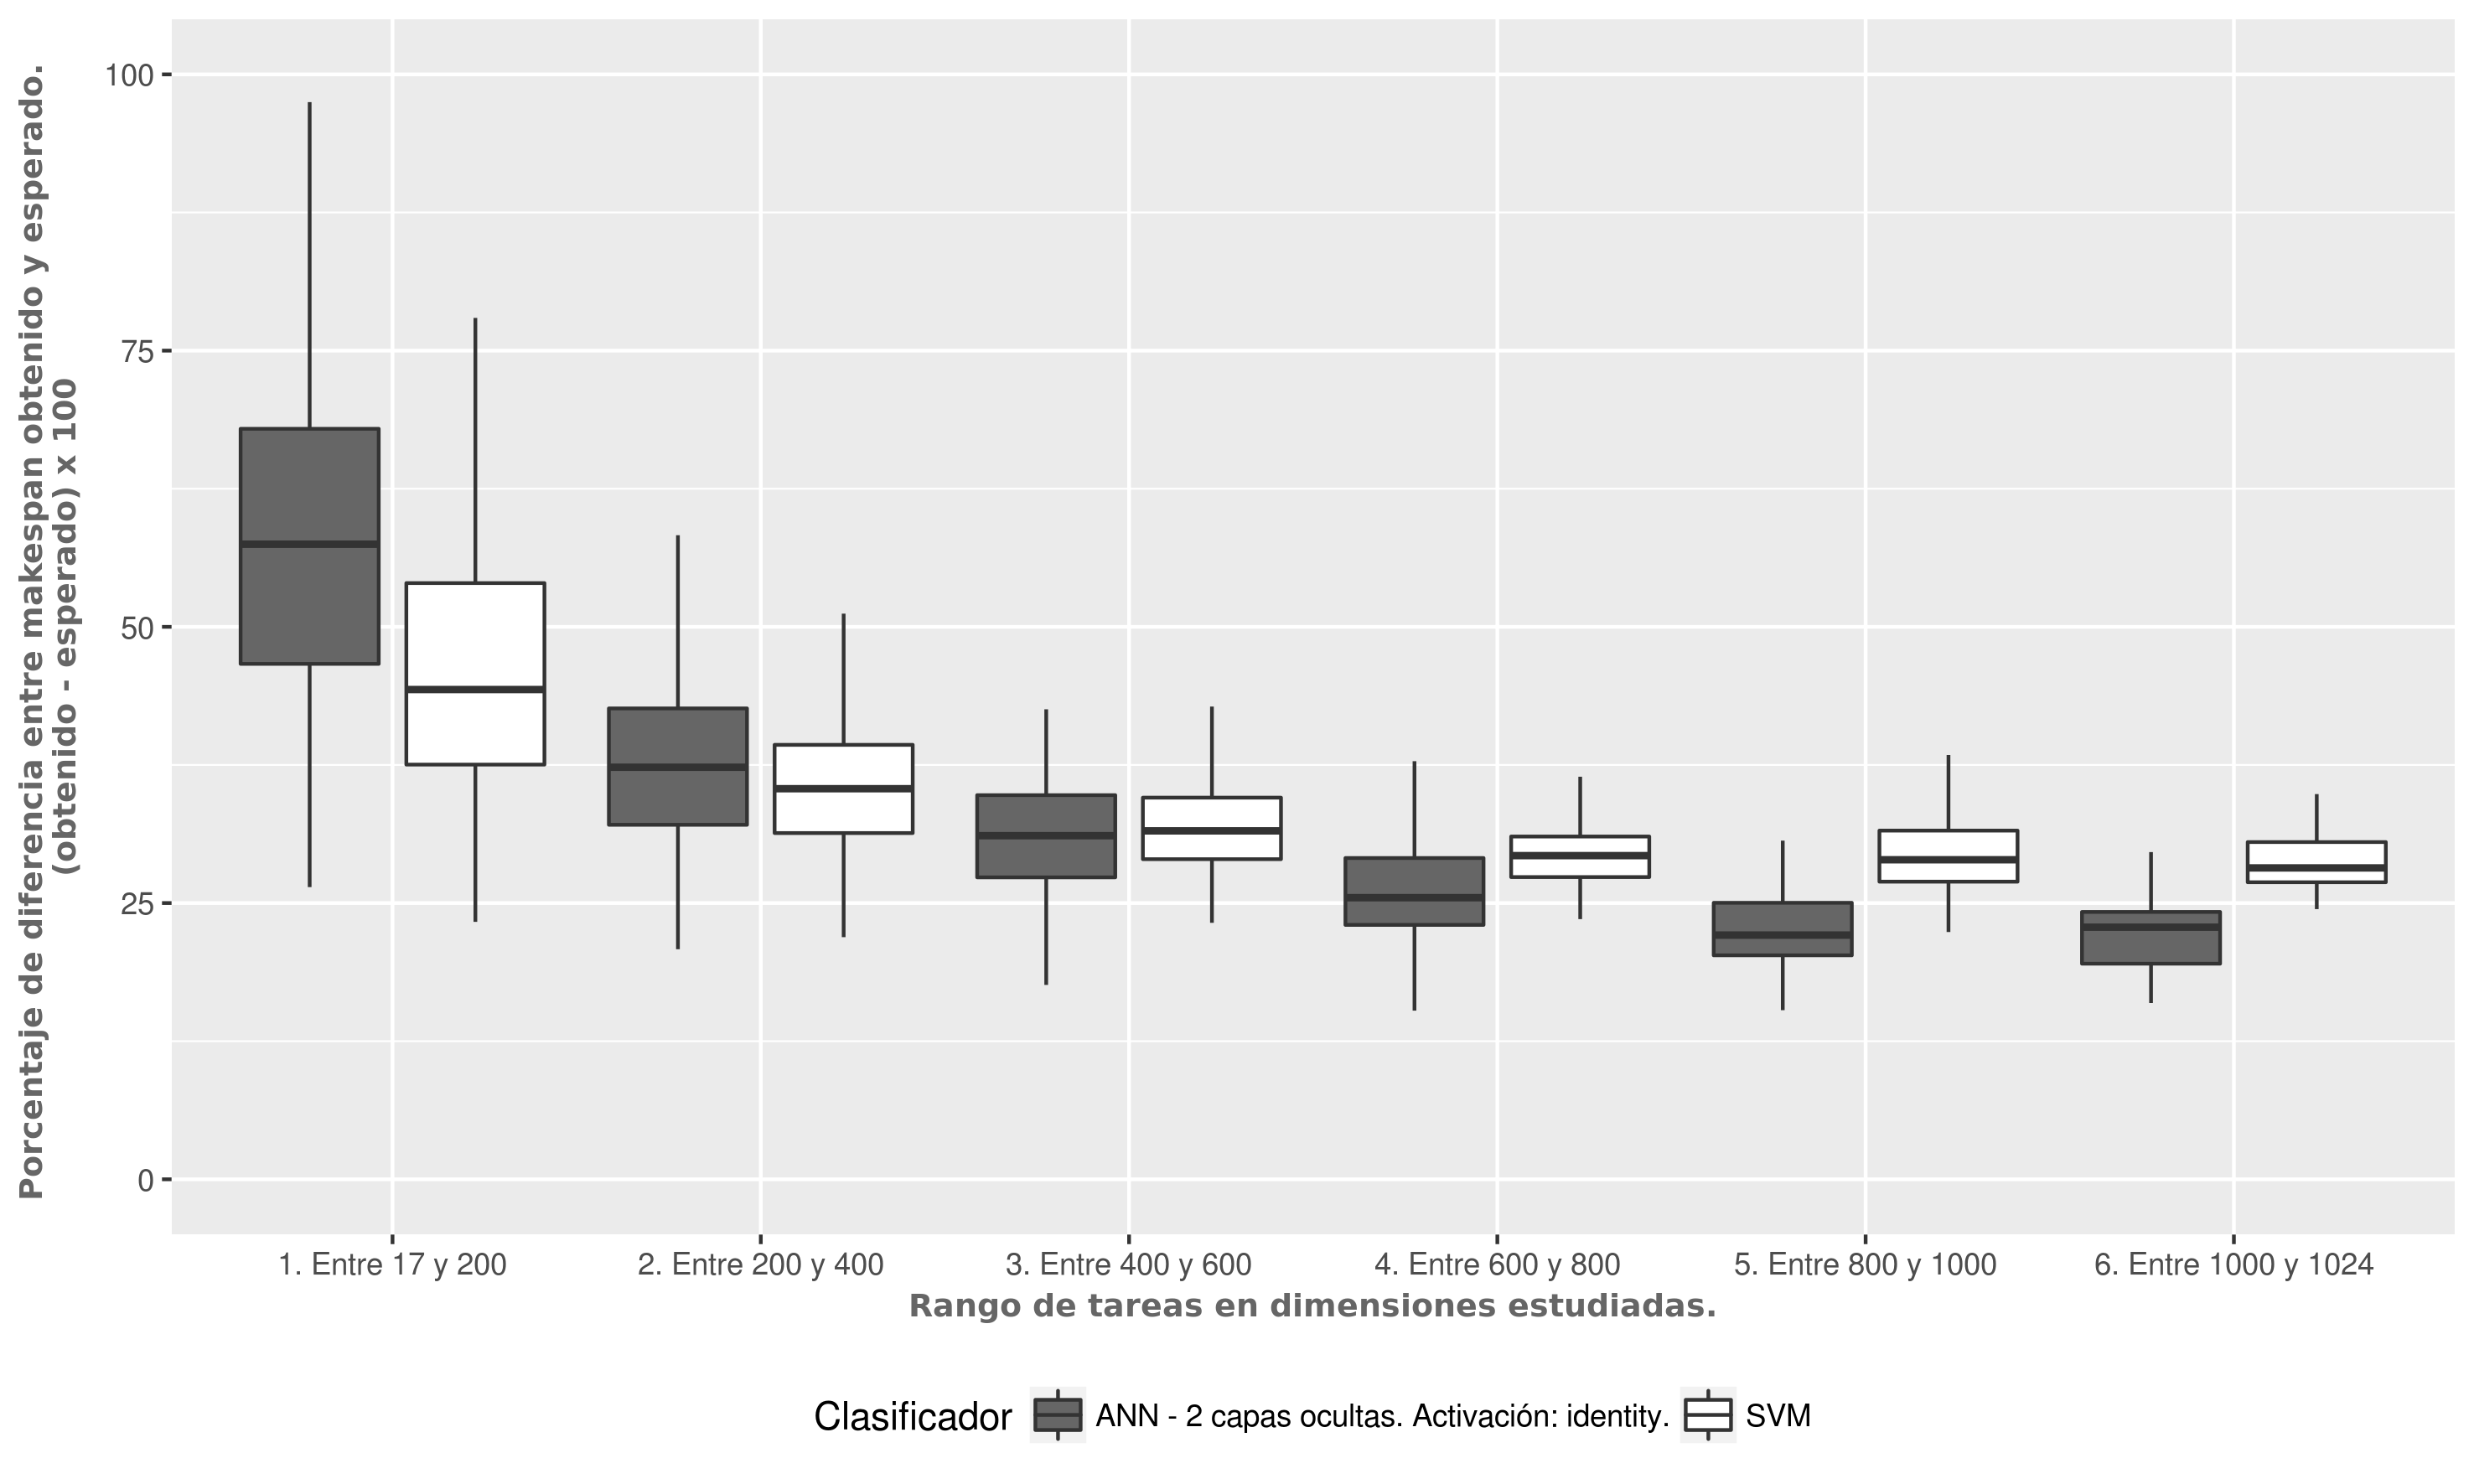
\includegraphics[width=\columnwidth]{imagenes/identity/2_medianas_diferenciasann_2_capas_ocultas_identity.png}
  \caption{Comparación de la diferencia porcentual de \textit{makespan} para la red neuronal con activación \textit{identity}, de dos capas ocultas con respecto a los valores esperados obtenidos con el algoritmo Min-Min.
Así también se muestran los resultados obtenidos para la SVM.
Los resultados se muestran divididos en rangos de dimensión desde $ 17 \times 16$ a $ 1024 \times 16$}
  \label{fig:identity_makespan}
\end{figure}

\newpage % orphaned line.

\begin{figure}[H]
  \centering
  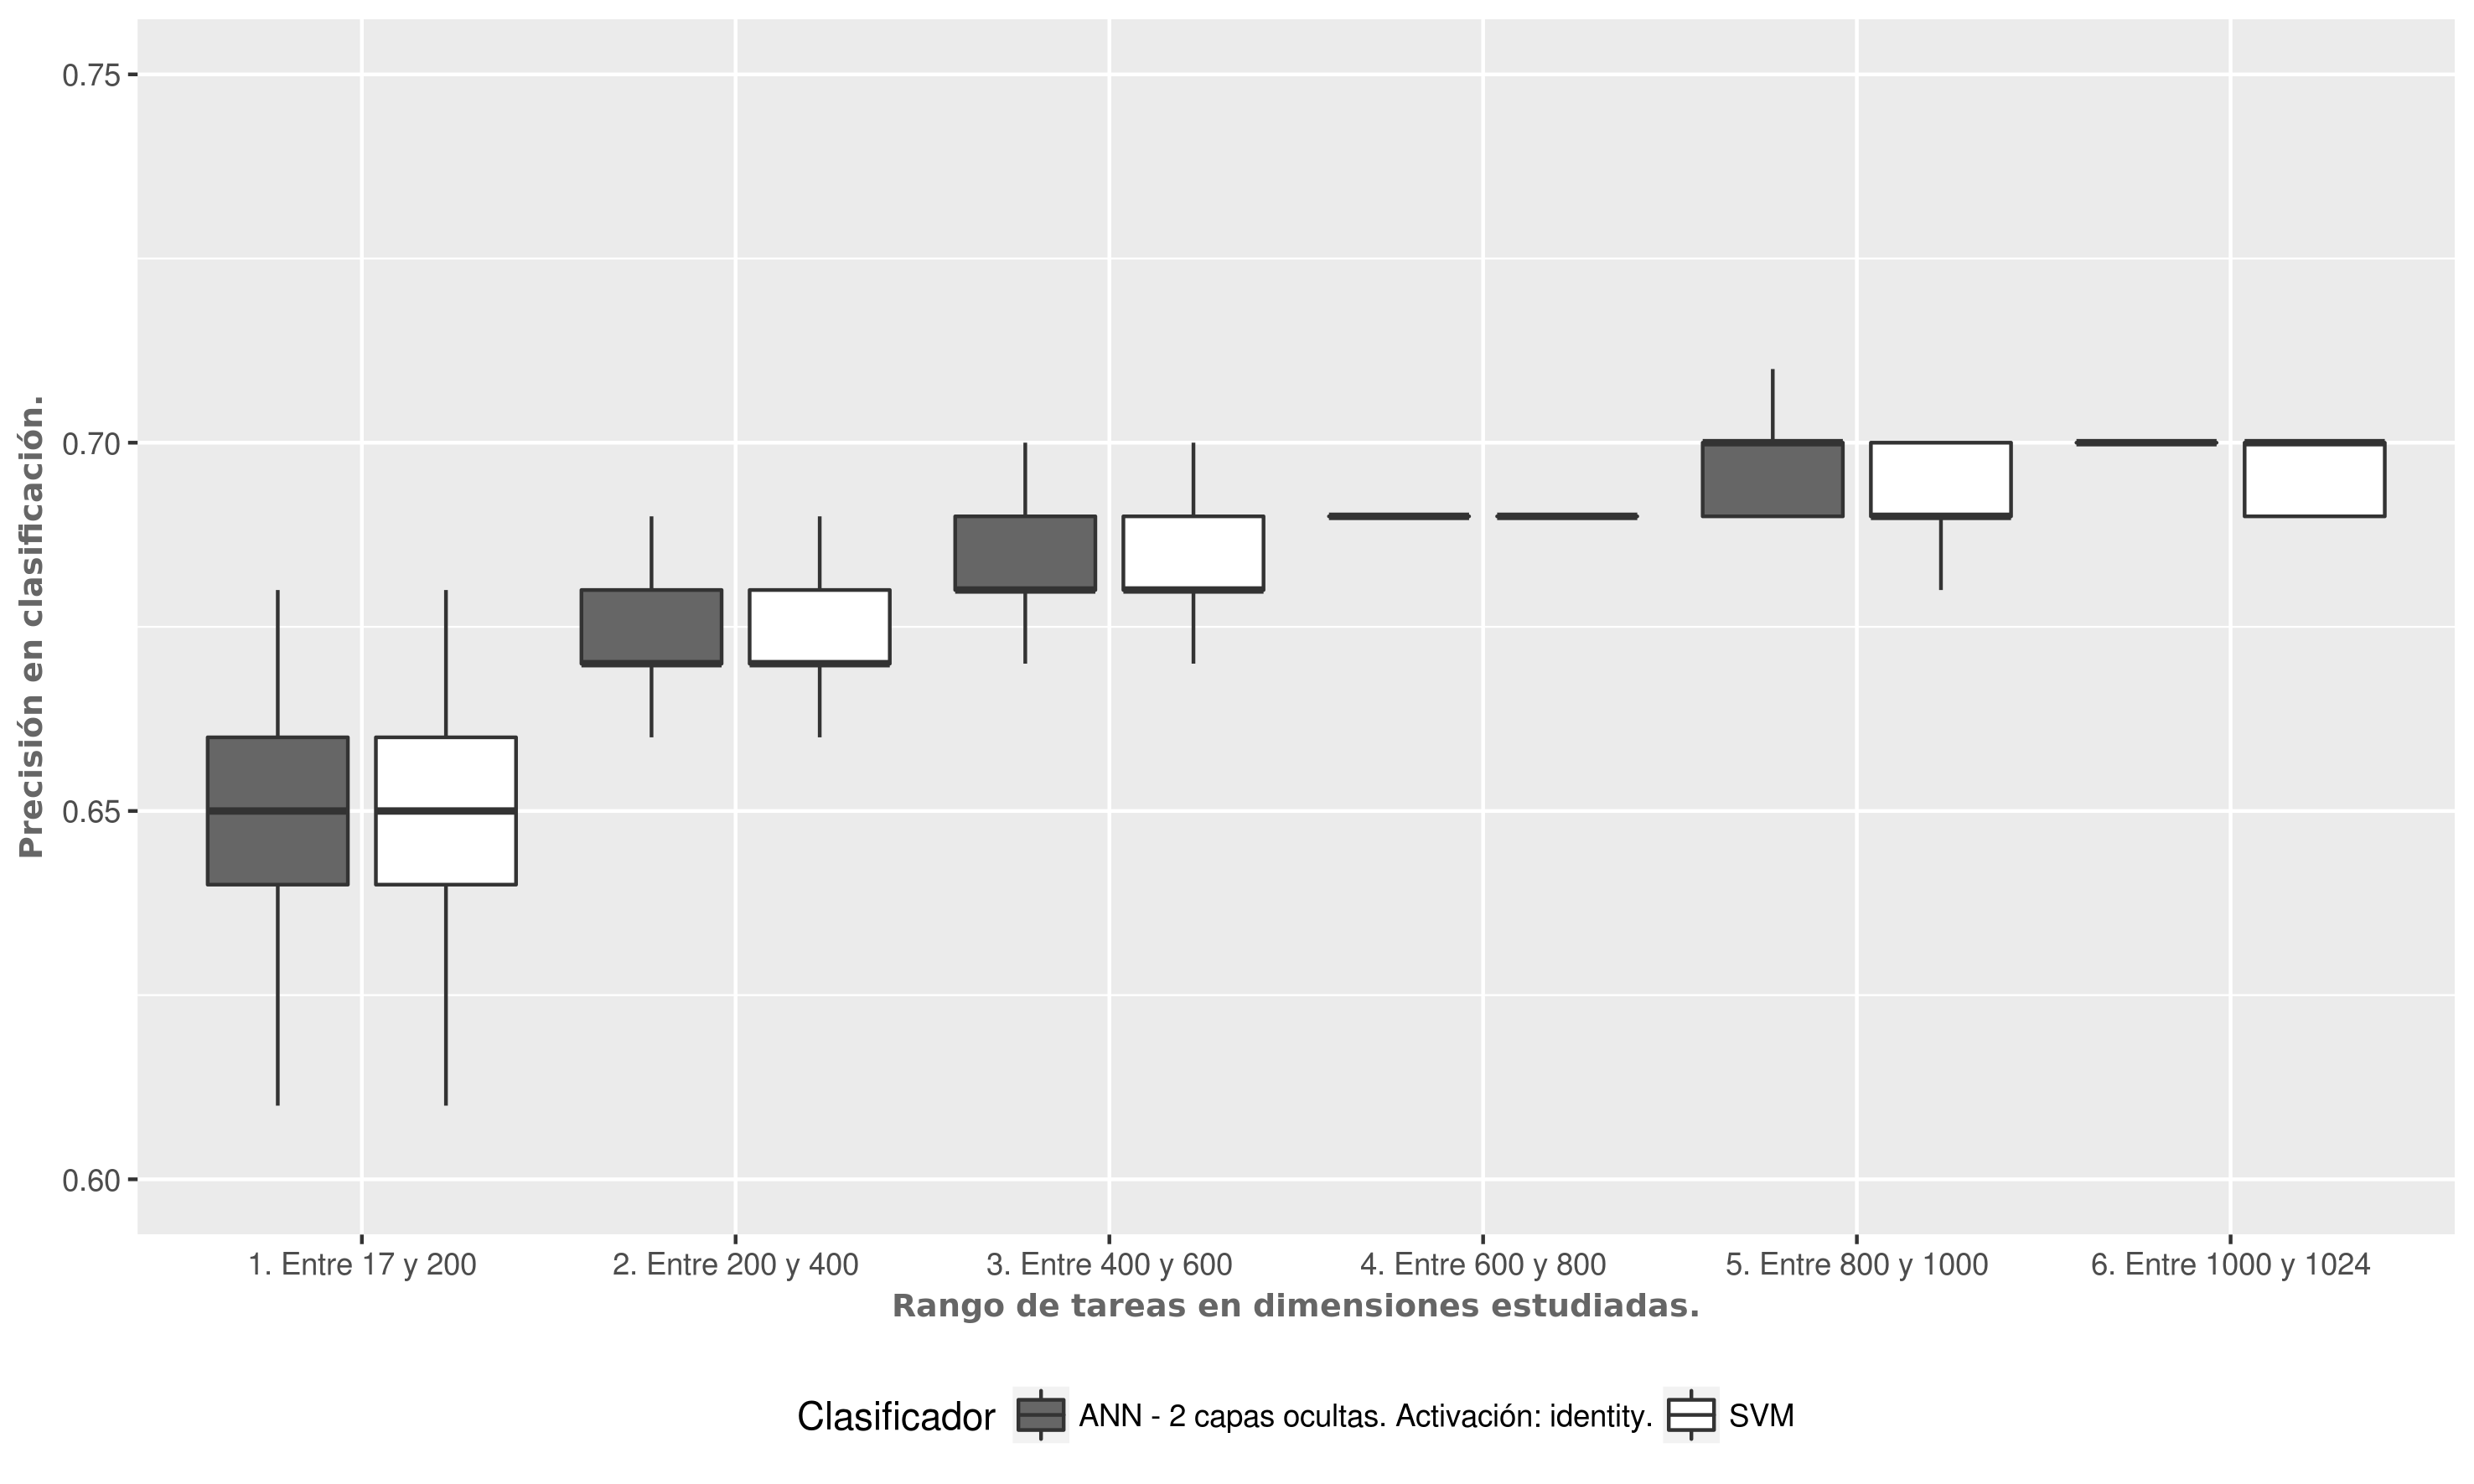
\includegraphics[width=\columnwidth]{imagenes/identity/3_accuracy_ann_2_capas_ocultas_identity.png}
  \caption{Precisión en clasificación para la red neuronal con función de activación \textit{identity} y para la SVM.
Los resultados se muestran divididos en rangos de dimensión desde $ 17 \times 16$ a $ 1024 \times 16$.}
  \label{fig:identity_accuracy}
\end{figure}

\paragraph{}Al observar el porcentaje de mejores máquinas seleccionadas frente a un error en la Figura \ref{fig:identity_mejores}, se observa que la red neuronal con función de activación \textit{identity} selecciona máquinas más rápidas en proporciones similares a la SVM, a diferencia de los resultados presentados para la red neuronal con función de activación \textit{relu}, que tiende a elegir máquinas más lentas que la SVM frente a un error.
Estos resultados llevan a pensar que el hecho de que la proporción de selección de mejores máquinas por parte de la red neuronal con función de activación \textit{identity} sea mayor que para el caso de \textit{relu}, conduce a una leve disminución del \textit{makespan}. 

\newpage % orphaned line.

\begin{figure}[H]
  \centering
  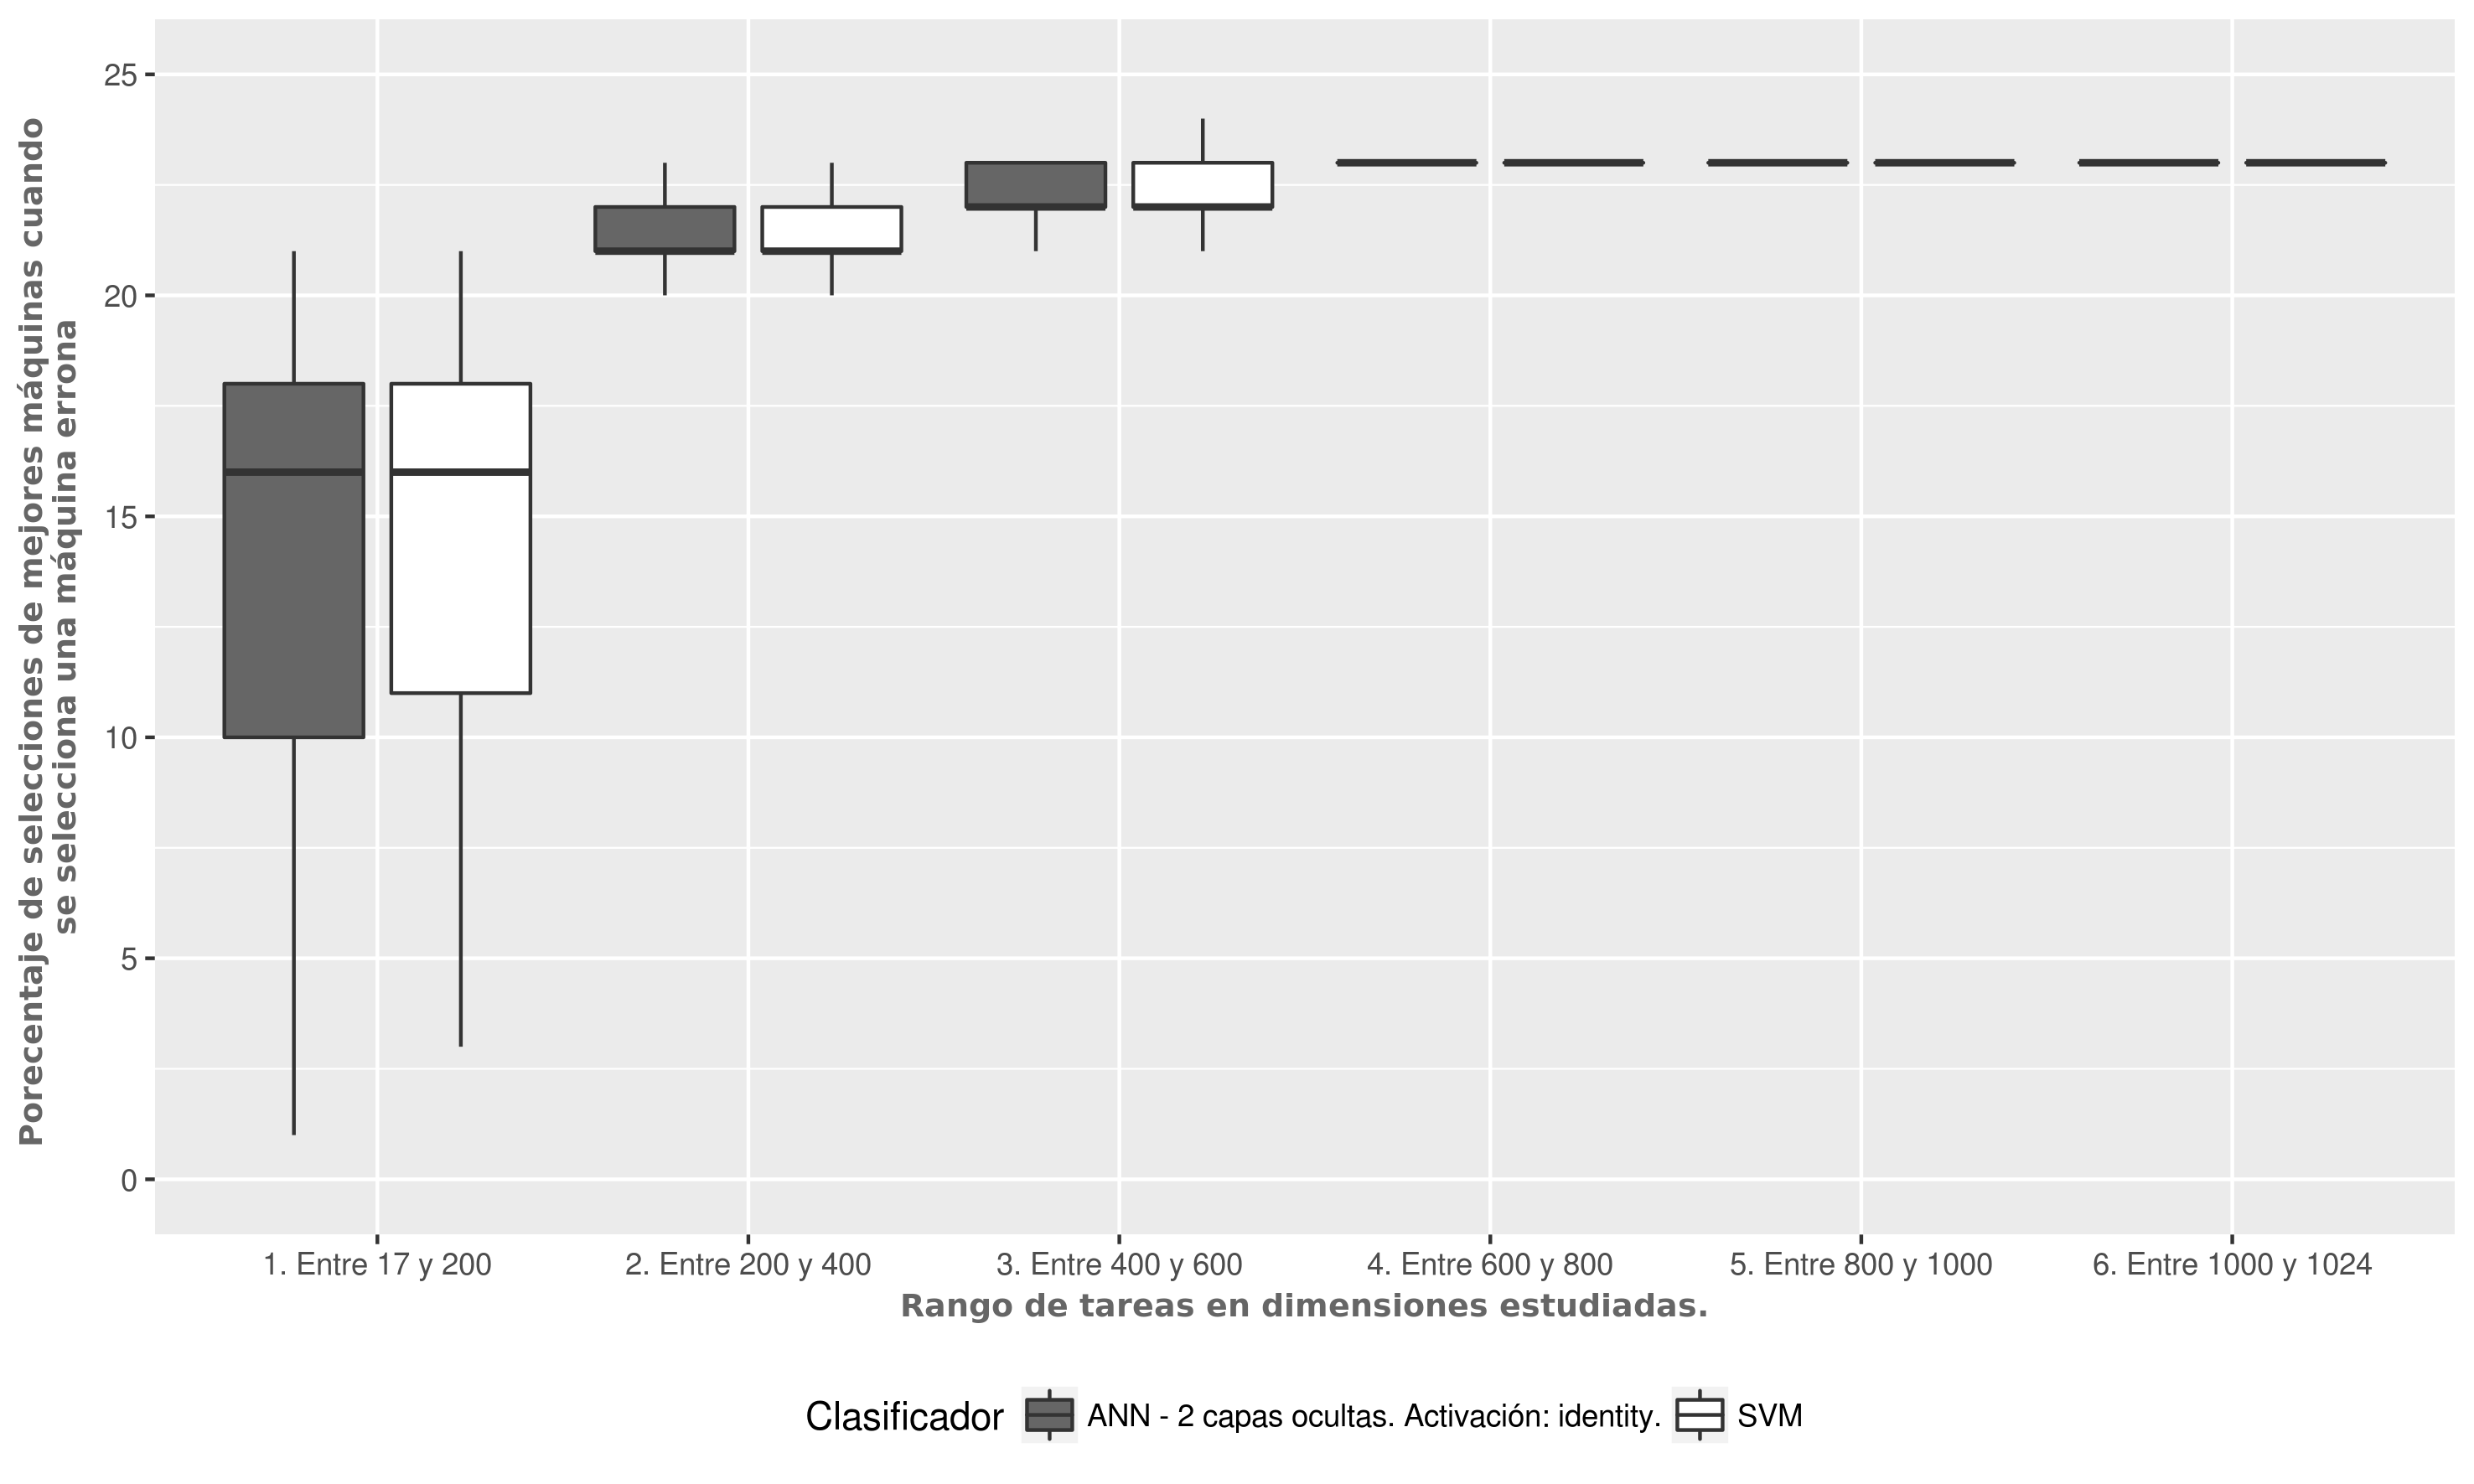
\includegraphics[width=\columnwidth]{imagenes/identity/4_porcentaje_maquinas_mejores_ann_2_capas_ocultas_identity.png}
  \caption{Porcentaje de selección de máquinas mejores frente a una selección diferente a la esperada para la red neuronal con activación \textit{identity} de dos capas ocultas y para la SVM.}
  \label{fig:identity_mejores}
\end{figure}

\newpage % orphaned line.

\section{Red neuronal con activación \textit{tanh} de dos capas ocultas}

La Figura \ref{fig:tanh_makespan} muestra las diferencias porcentuales de \textit{makespan} para la red neuronal con activación \textit{tanh} y para la SVM.
En esta se observa una leve mejora en \textit{makespan} para la red neuronal con respecto al \textit{makespan} obtenido con SVM, para dimensiones grandes.
Esta mejora va acompañada de una mejora en la precisión, sustancial en comparación con las precisiones de las otras funciones de activación estudiadas, como se observa en la Figura \ref{fig:tanh_accuracy}.

\begin{figure}[H]
  \centering
  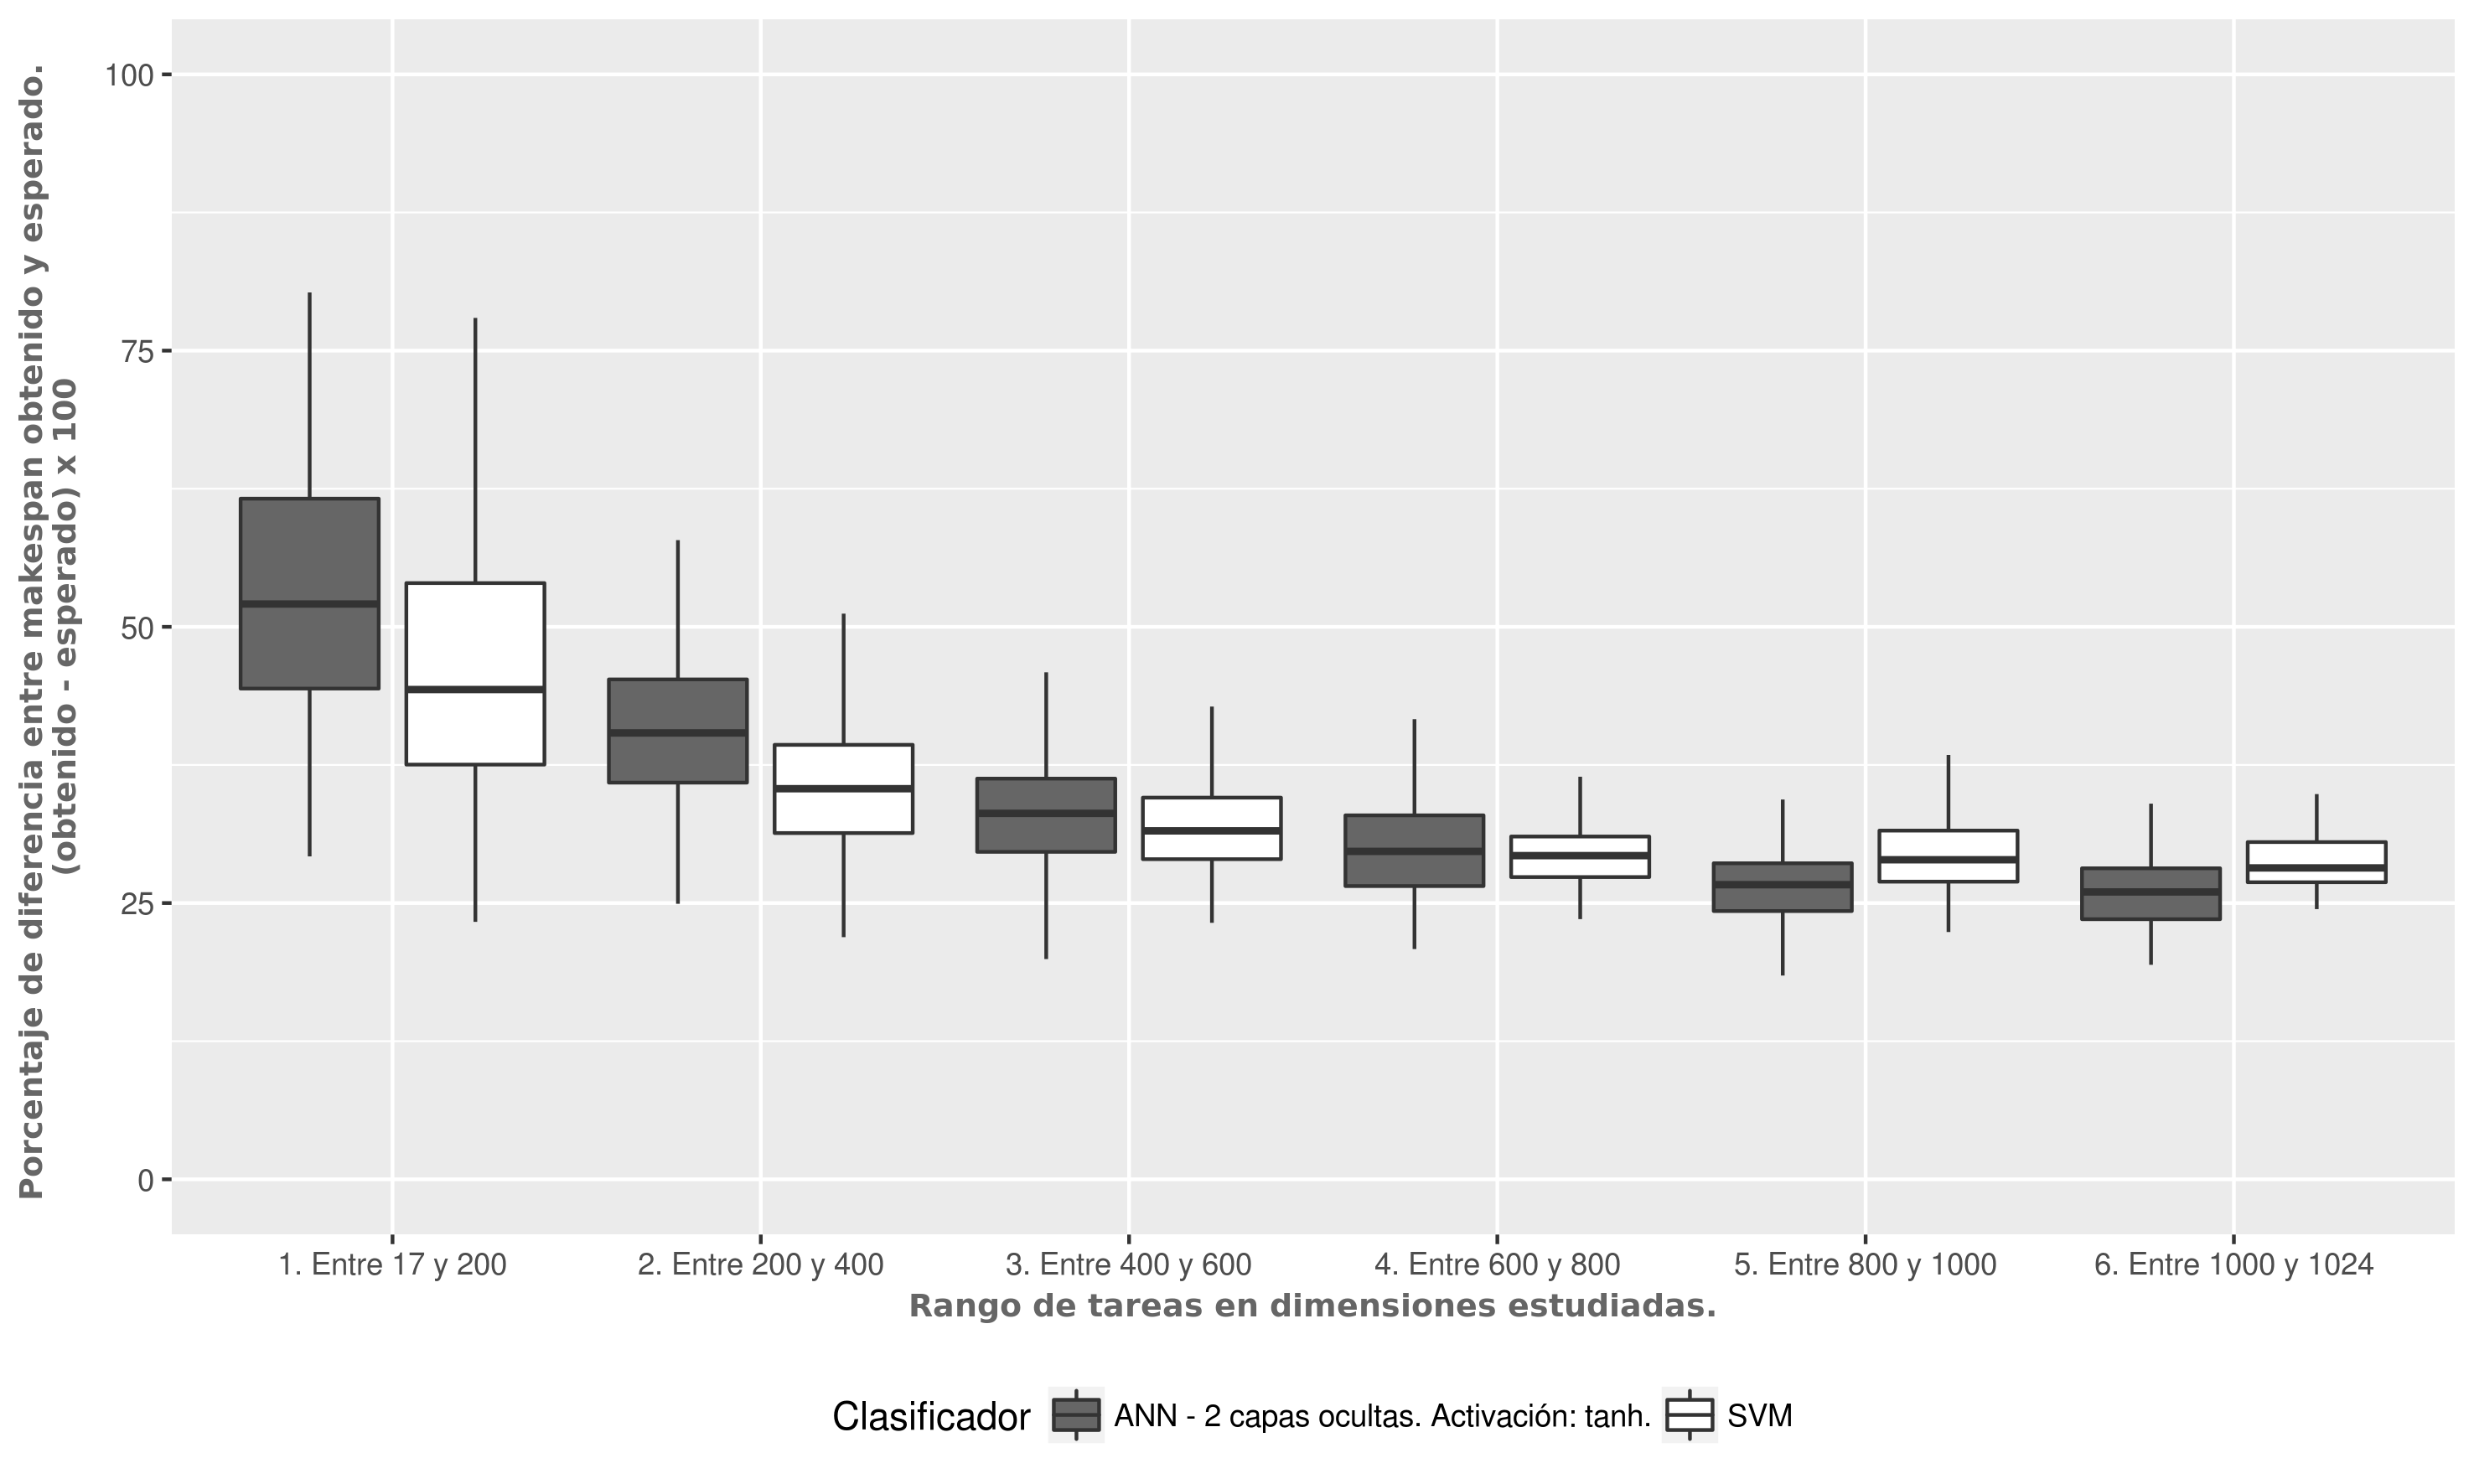
\includegraphics[width=\columnwidth]{imagenes/tanh/2_medianas_diferenciasann_2_capas_ocultas_tanh.png}
  \caption{Comparación de la diferencia porcentual de \textit{makespan} para la red neuronal con activación \textit{tanh}, de dos capas ocultas con respecto a los valores esperados obtenidos con el algoritmo Min-Min.
Así también se muestran los resultados obtenidos para la SVM.
Los resultados se muestran divididos en rangos de dimensión desde $ 17 \times 16$ a $ 1024 \times 16$}
  \label{fig:tanh_makespan}
\end{figure}

\newpage % orphaned line.

\begin{figure}[H]
  \centering
  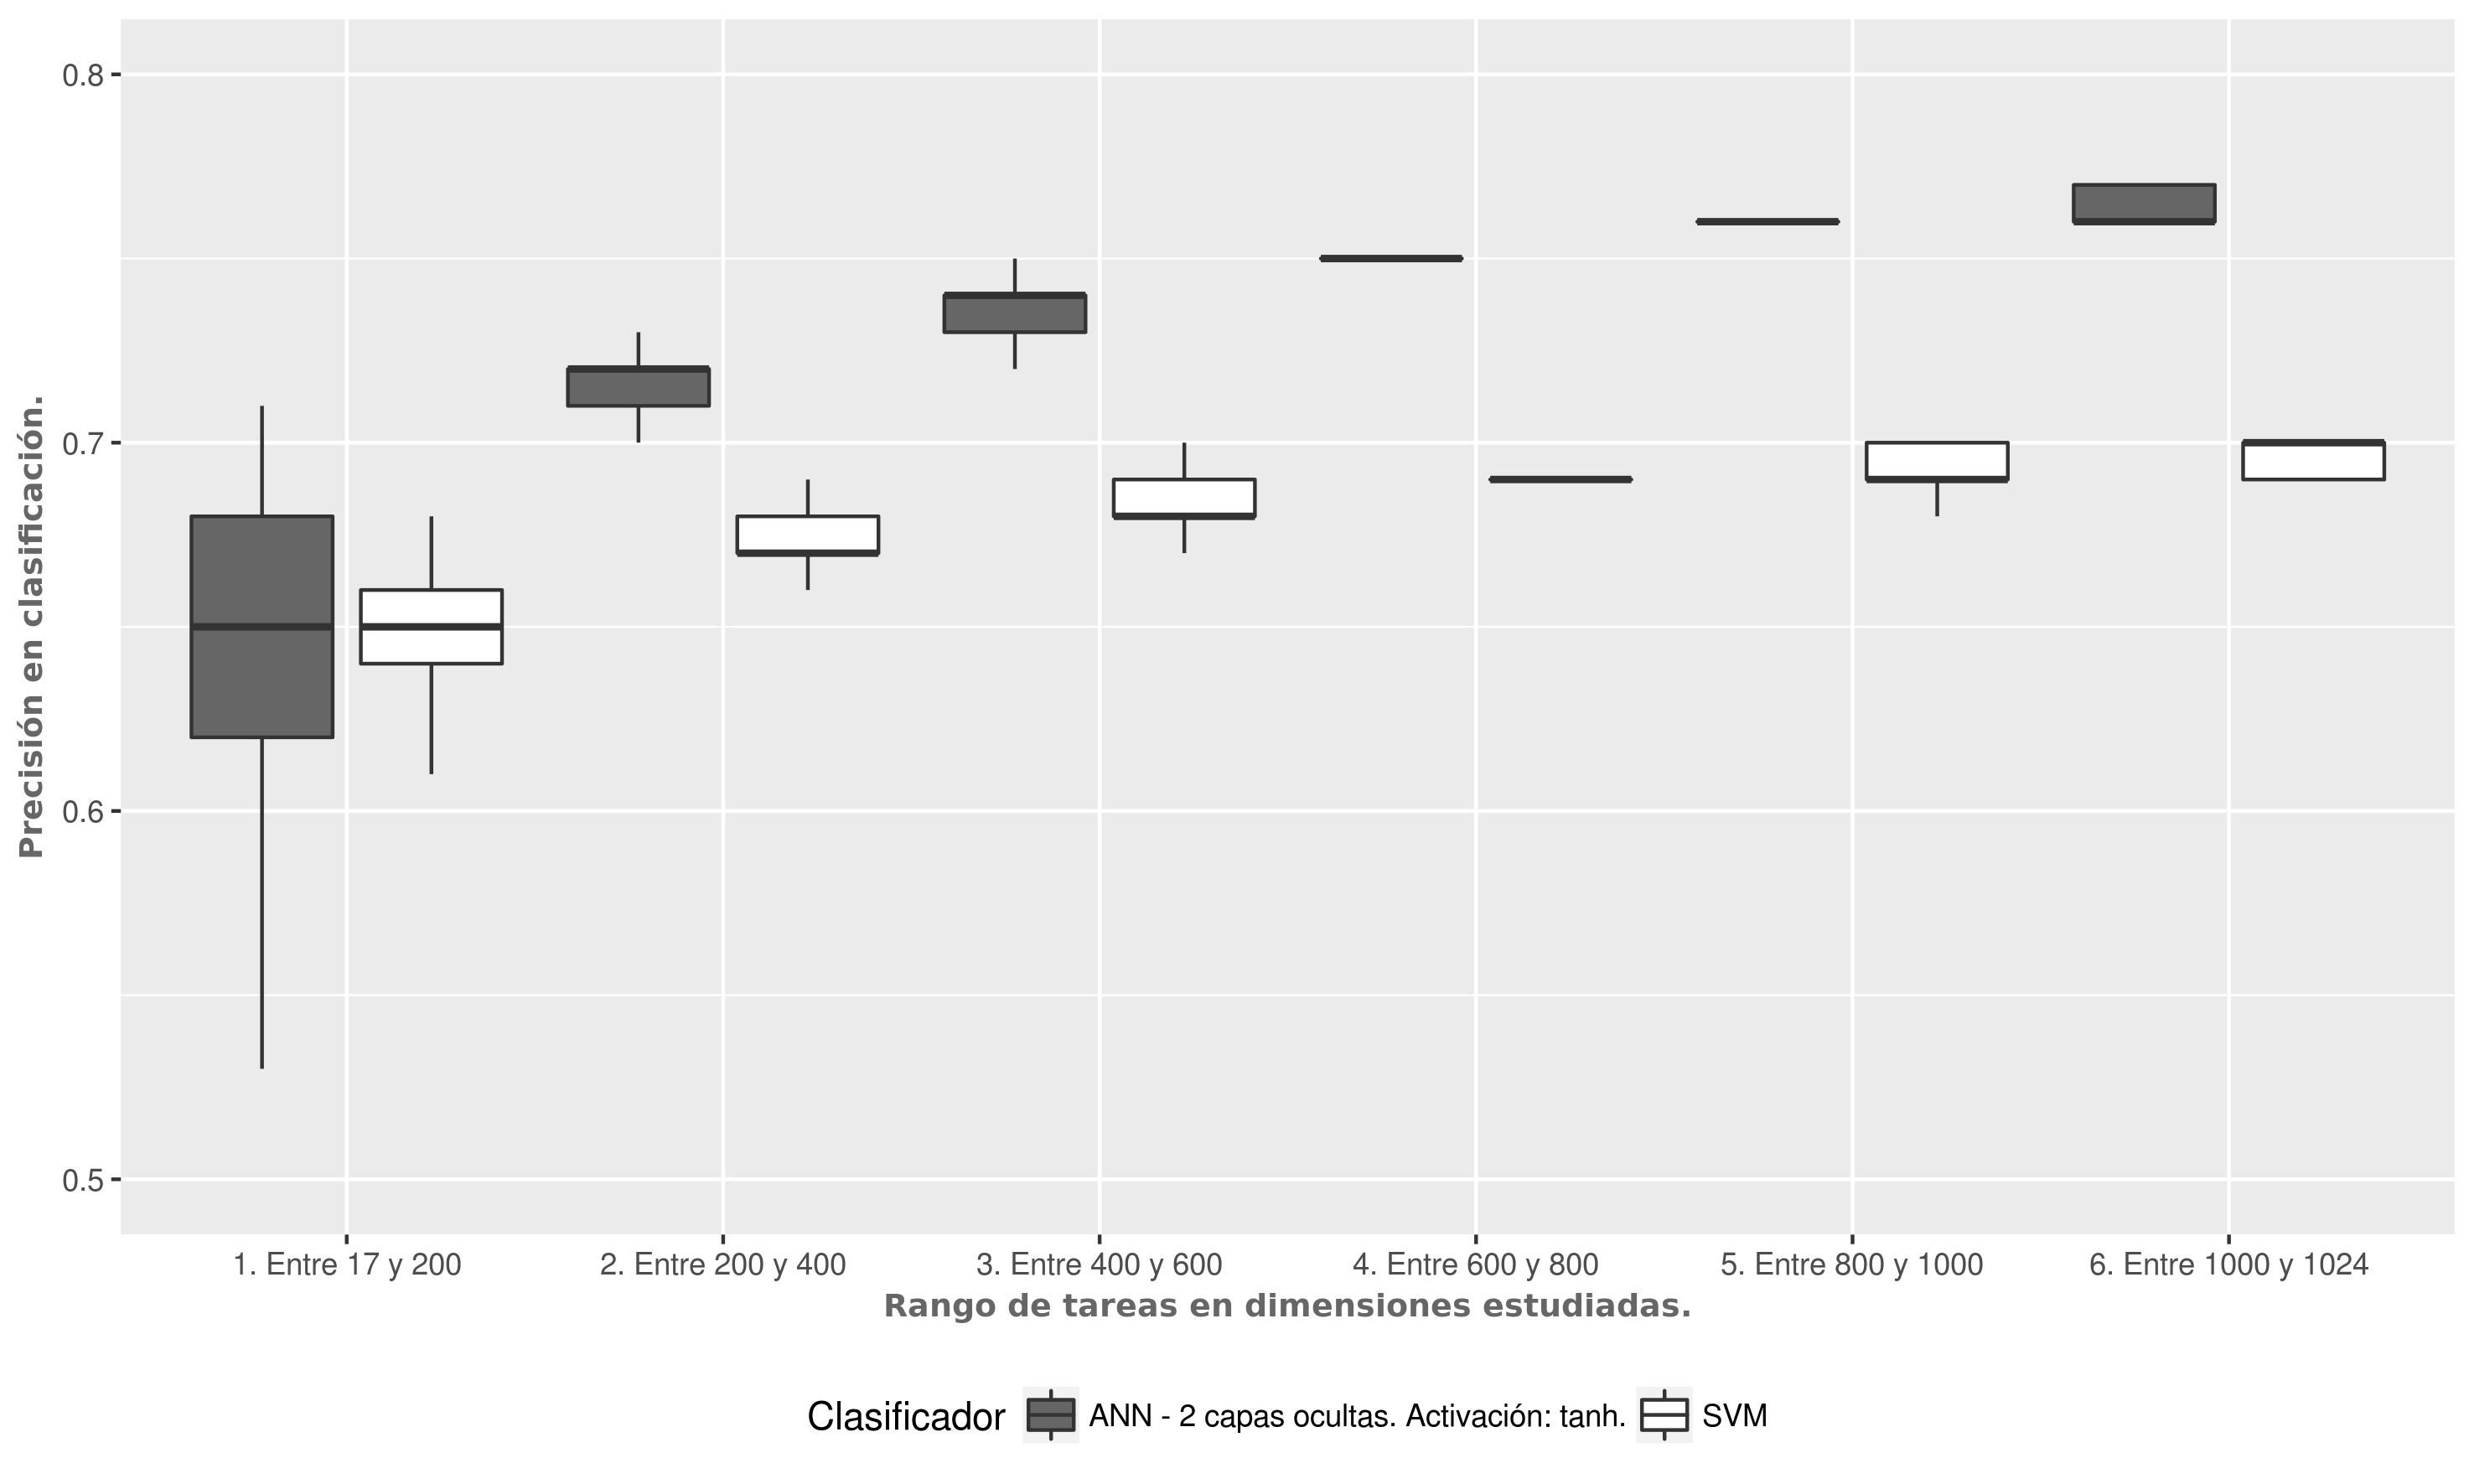
\includegraphics[width=\columnwidth]{imagenes/tanh/3_accuracy_ann_2_capas_ocultas_tanh.png}
  \caption{Precisión en clasificación para la red neuronal con función de activación \textit{tanh} y para la SVM.
Los resultados se muestran divididos en rangos de dimensión desde $ 17 \times 16$ a $ 1024 \times 16$.}
  \label{fig:tanh_accuracy}
\end{figure}

\paragraph{} La Figura \ref{fig:tanh_mejores} muestra que la red neuronal con función de activación \textit{tanh} selecciona máquinas más lentas que SVM cuando se selecciona una máquina diferente a la esperada.

\paragraph{} Para dimensiones grandes se selecciona alrededor de un $15\%$ de mejores máquinas para la función de activación \textit{tanh}, siendo este porcentaje el más bajo obtenido para todas las funciones de activación estudiadas.
Esto conduce a pensar que la precisión es fundamental para aproximarse al \textit{makespan} esperado y que las decisiones que se toman a la hora de seleccionar una máquina diferente a la esperada pierde importancia frente a una precisión elevada en clasificación, donde un error puede costar caro en términos de tiempos de ejecución o \textit{makespan}.

\newpage % orphaned line.

\begin{figure}[H]
  \centering
  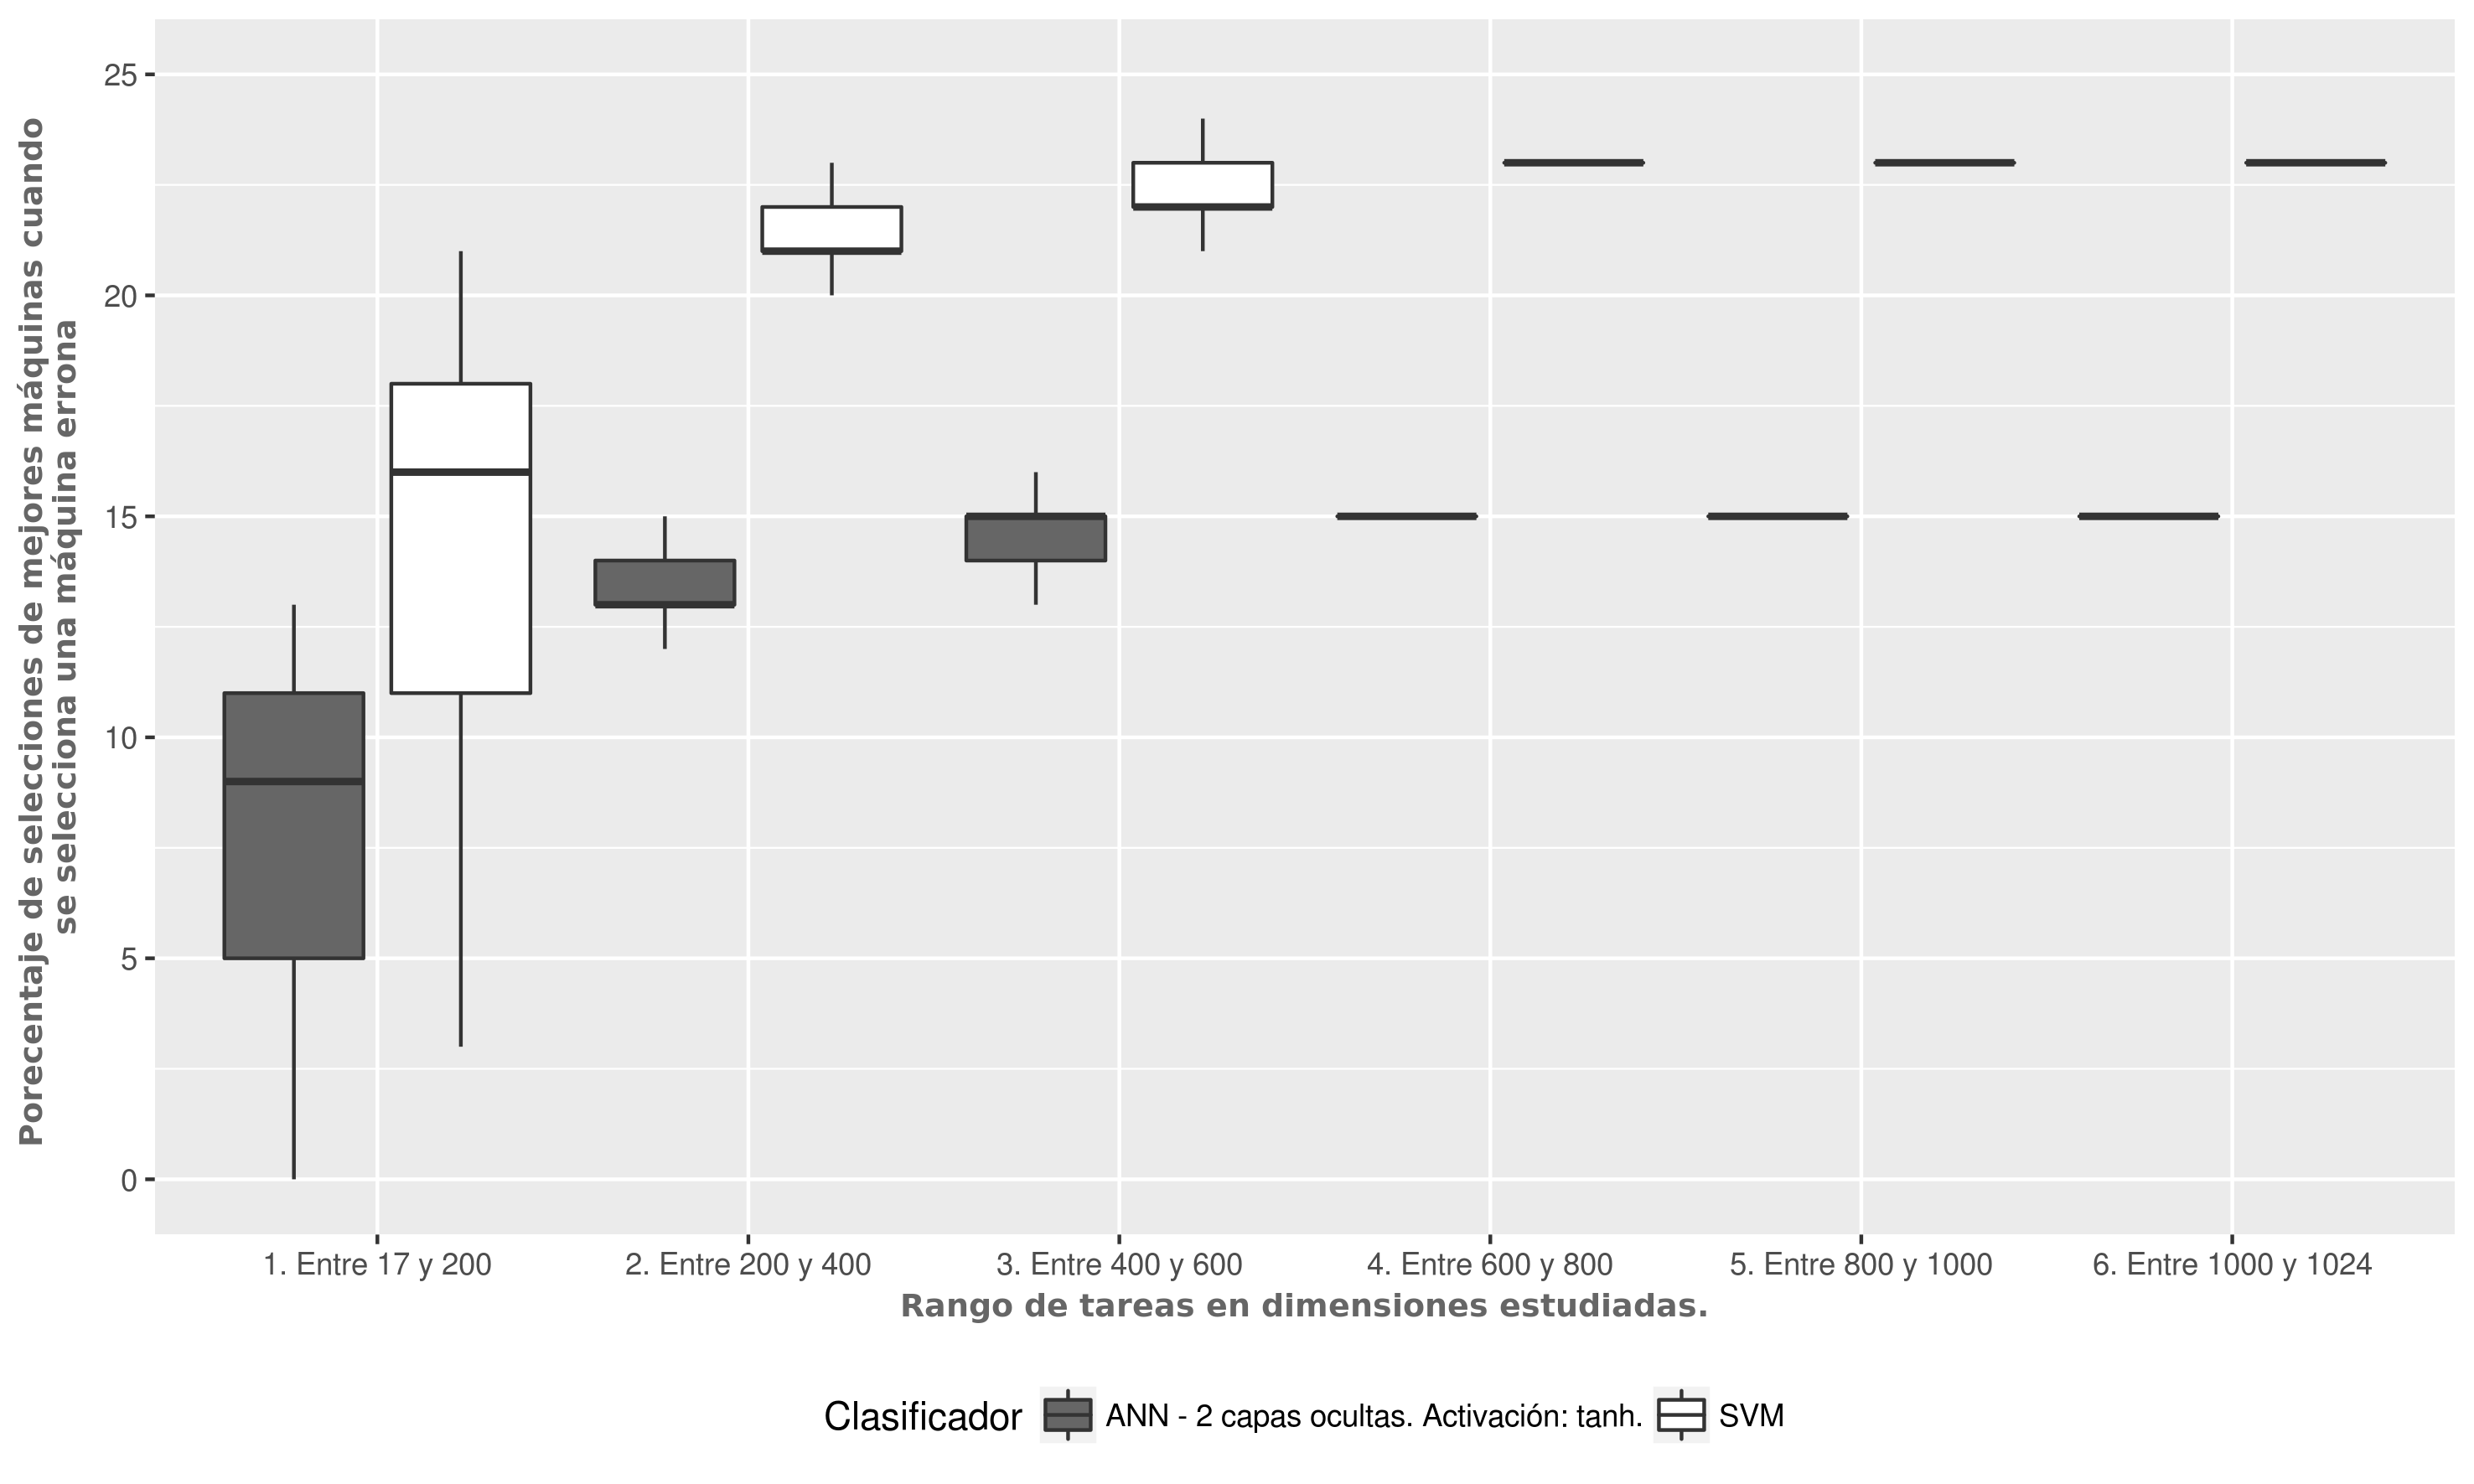
\includegraphics[width=\columnwidth]{imagenes/tanh/4_porcentaje_maquinas_mejores_ann_2_capas_ocultas_tanh.png}
  \caption{Porcentaje de selección de máquinas mejores frente a una selección diferente a la esperada para la red neuronal con activación \textit{tanh} de dos capas ocultas y para la SVM.}
  \label{fig:tanh_mejores}
\end{figure}

\newpage % orphaned line.

\section{Observaciones generales}

\paragraph{} En términos generales, entrenar redes neuronales con menor cantidad de capas ocultas, generó mejores resultados de \textit{makespan} en clasificación, que entrenar redes neuronales con mayor cantidad de capas ocultas.
Esto se traduce en mejores resultados de \textit{makespan} con una menor inversión en tiempo de entrenamiento. 

\paragraph{} Para redes neuronales entrenadas utilizando \textit{tanh} e \textit{identity} como funciones de activación, el \textit{makespan} de los resultados mejoró levemente con respecto al \textit{makespan} de los resultados obtenidos con SVM para dimensiones grandes del problema.
Se observó una relación directa entre la precisión y la mejora porcentual de \textit{makespan} para la red neuronal con activación \textit{tanh}. También se observó una relación entre el porcentaje de selección de mejores máquinas frente a un error y la mejora porcentual de \textit{makespan}, donde una buena selección de máquina frente a un error en la clasificación, puede mitigar los efectos negativos sobre el \textit{makespan} que genera tener una precisión baja. La red neuronal de dos capas ocultas con función de activación \textit{tanh} obtuvo resultados similares en cuanto a \textit{makespan} que la red neuronal de dos capas ocultas con función de activación \textit{identity}, pero la primera obtuvo mejores valores de precisión en clasificación, lo cual hace de la red neuronal con activación \textit{tanh} una configuración de red neuronal potencialmente adecuada para aprender a resolver el problema HCSP.

\paragraph{} Los resultados obtenidos con la red neuronal con función de activación \textit{relu} no mejoraron los resultados obtenidos con SVM en términos de \textit{makespan}, obteniendo precisiones en clasificación similares, teniendo un porcentaje menor de selección de mejores máquinas frente a un error. Esto hace que \textit{relu} sea una función de activación poco adecuada si el objetivo perseguido es aprender a resolver el problema HCSP.